% Options for packages loaded elsewhere
\PassOptionsToPackage{unicode}{hyperref}
\PassOptionsToPackage{hyphens}{url}
\documentclass[
]{article}
\usepackage{xcolor}
\usepackage{amsmath,amssymb}
\setcounter{secnumdepth}{-\maxdimen} % remove section numbering
\usepackage{iftex}
\ifPDFTeX
  \usepackage[T1]{fontenc}
  \usepackage[utf8]{inputenc}
  \usepackage{textcomp} % provide euro and other symbols
\else % if luatex or xetex
  \usepackage{unicode-math} % this also loads fontspec
  \defaultfontfeatures{Scale=MatchLowercase}
  \defaultfontfeatures[\rmfamily]{Ligatures=TeX,Scale=1}
\fi
\usepackage{lmodern}
\ifPDFTeX\else
  % xetex/luatex font selection
\fi
% Use upquote if available, for straight quotes in verbatim environments
\IfFileExists{upquote.sty}{\usepackage{upquote}}{}
\IfFileExists{microtype.sty}{% use microtype if available
  \usepackage[]{microtype}
  \UseMicrotypeSet[protrusion]{basicmath} % disable protrusion for tt fonts
}{}
\makeatletter
\@ifundefined{KOMAClassName}{% if non-KOMA class
  \IfFileExists{parskip.sty}{%
    \usepackage{parskip}
  }{% else
    \setlength{\parindent}{0pt}
    \setlength{\parskip}{6pt plus 2pt minus 1pt}}
}{% if KOMA class
  \KOMAoptions{parskip=half}}
\makeatother
\usepackage{color}
\usepackage{fancyvrb}
\newcommand{\VerbBar}{|}
\newcommand{\VERB}{\Verb[commandchars=\\\{\}]}
\DefineVerbatimEnvironment{Highlighting}{Verbatim}{commandchars=\\\{\}}
% Add ',fontsize=\small' for more characters per line
\newenvironment{Shaded}{}{}
\newcommand{\AlertTok}[1]{\textcolor[rgb]{1.00,0.00,0.00}{\textbf{#1}}}
\newcommand{\AnnotationTok}[1]{\textcolor[rgb]{0.38,0.63,0.69}{\textbf{\textit{#1}}}}
\newcommand{\AttributeTok}[1]{\textcolor[rgb]{0.49,0.56,0.16}{#1}}
\newcommand{\BaseNTok}[1]{\textcolor[rgb]{0.25,0.63,0.44}{#1}}
\newcommand{\BuiltInTok}[1]{\textcolor[rgb]{0.00,0.50,0.00}{#1}}
\newcommand{\CharTok}[1]{\textcolor[rgb]{0.25,0.44,0.63}{#1}}
\newcommand{\CommentTok}[1]{\textcolor[rgb]{0.38,0.63,0.69}{\textit{#1}}}
\newcommand{\CommentVarTok}[1]{\textcolor[rgb]{0.38,0.63,0.69}{\textbf{\textit{#1}}}}
\newcommand{\ConstantTok}[1]{\textcolor[rgb]{0.53,0.00,0.00}{#1}}
\newcommand{\ControlFlowTok}[1]{\textcolor[rgb]{0.00,0.44,0.13}{\textbf{#1}}}
\newcommand{\DataTypeTok}[1]{\textcolor[rgb]{0.56,0.13,0.00}{#1}}
\newcommand{\DecValTok}[1]{\textcolor[rgb]{0.25,0.63,0.44}{#1}}
\newcommand{\DocumentationTok}[1]{\textcolor[rgb]{0.73,0.13,0.13}{\textit{#1}}}
\newcommand{\ErrorTok}[1]{\textcolor[rgb]{1.00,0.00,0.00}{\textbf{#1}}}
\newcommand{\ExtensionTok}[1]{#1}
\newcommand{\FloatTok}[1]{\textcolor[rgb]{0.25,0.63,0.44}{#1}}
\newcommand{\FunctionTok}[1]{\textcolor[rgb]{0.02,0.16,0.49}{#1}}
\newcommand{\ImportTok}[1]{\textcolor[rgb]{0.00,0.50,0.00}{\textbf{#1}}}
\newcommand{\InformationTok}[1]{\textcolor[rgb]{0.38,0.63,0.69}{\textbf{\textit{#1}}}}
\newcommand{\KeywordTok}[1]{\textcolor[rgb]{0.00,0.44,0.13}{\textbf{#1}}}
\newcommand{\NormalTok}[1]{#1}
\newcommand{\OperatorTok}[1]{\textcolor[rgb]{0.40,0.40,0.40}{#1}}
\newcommand{\OtherTok}[1]{\textcolor[rgb]{0.00,0.44,0.13}{#1}}
\newcommand{\PreprocessorTok}[1]{\textcolor[rgb]{0.74,0.48,0.00}{#1}}
\newcommand{\RegionMarkerTok}[1]{#1}
\newcommand{\SpecialCharTok}[1]{\textcolor[rgb]{0.25,0.44,0.63}{#1}}
\newcommand{\SpecialStringTok}[1]{\textcolor[rgb]{0.73,0.40,0.53}{#1}}
\newcommand{\StringTok}[1]{\textcolor[rgb]{0.25,0.44,0.63}{#1}}
\newcommand{\VariableTok}[1]{\textcolor[rgb]{0.10,0.09,0.49}{#1}}
\newcommand{\VerbatimStringTok}[1]{\textcolor[rgb]{0.25,0.44,0.63}{#1}}
\newcommand{\WarningTok}[1]{\textcolor[rgb]{0.38,0.63,0.69}{\textbf{\textit{#1}}}}
\usepackage{longtable,booktabs,array}
\usepackage{calc} % for calculating minipage widths
% Correct order of tables after \paragraph or \subparagraph
\usepackage{etoolbox}
\makeatletter
\patchcmd\longtable{\par}{\if@noskipsec\mbox{}\fi\par}{}{}
\makeatother
% Allow footnotes in longtable head/foot
\IfFileExists{footnotehyper.sty}{\usepackage{footnotehyper}}{\usepackage{footnote}}
\makesavenoteenv{longtable}
\usepackage{graphicx}
\makeatletter
\newsavebox\pandoc@box
\newcommand*\pandocbounded[1]{% scales image to fit in text height/width
  \sbox\pandoc@box{#1}%
  \Gscale@div\@tempa{\textheight}{\dimexpr\ht\pandoc@box+\dp\pandoc@box\relax}%
  \Gscale@div\@tempb{\linewidth}{\wd\pandoc@box}%
  \ifdim\@tempb\p@<\@tempa\p@\let\@tempa\@tempb\fi% select the smaller of both
  \ifdim\@tempa\p@<\p@\scalebox{\@tempa}{\usebox\pandoc@box}%
  \else\usebox{\pandoc@box}%
  \fi%
}
% Set default figure placement to htbp
\def\fps@figure{htbp}
\makeatother
\usepackage{svg}
% definitions for citeproc citations
\NewDocumentCommand\citeproctext{}{}
\NewDocumentCommand\citeproc{mm}{%
  \begingroup\def\citeproctext{#2}\cite{#1}\endgroup}
\makeatletter
 % allow citations to break across lines
 \let\@cite@ofmt\@firstofone
 % avoid brackets around text for \cite:
 \def\@biblabel#1{}
 \def\@cite#1#2{{#1\if@tempswa , #2\fi}}
\makeatother
\newlength{\cslhangindent}
\setlength{\cslhangindent}{1.5em}
\newlength{\csllabelwidth}
\setlength{\csllabelwidth}{3em}
\newenvironment{CSLReferences}[2] % #1 hanging-indent, #2 entry-spacing
 {\begin{list}{}{%
  \setlength{\itemindent}{0pt}
  \setlength{\leftmargin}{0pt}
  \setlength{\parsep}{0pt}
  % turn on hanging indent if param 1 is 1
  \ifodd #1
   \setlength{\leftmargin}{\cslhangindent}
   \setlength{\itemindent}{-1\cslhangindent}
  \fi
  % set entry spacing
  \setlength{\itemsep}{#2\baselineskip}}}
 {\end{list}}
\usepackage{calc}
\newcommand{\CSLBlock}[1]{\hfill\break\parbox[t]{\linewidth}{\strut\ignorespaces#1\strut}}
\newcommand{\CSLLeftMargin}[1]{\parbox[t]{\csllabelwidth}{\strut#1\strut}}
\newcommand{\CSLRightInline}[1]{\parbox[t]{\linewidth - \csllabelwidth}{\strut#1\strut}}
\newcommand{\CSLIndent}[1]{\hspace{\cslhangindent}#1}
\ifLuaTeX
\usepackage[bidi=basic]{babel}
\else
\usepackage[bidi=default]{babel}
\fi
\babelprovide[main,import]{french}
% get rid of language-specific shorthands (see #6817):
\let\LanguageShortHands\languageshorthands
\def\languageshorthands#1{}
\setlength{\emergencystretch}{3em} % prevent overfull lines
\providecommand{\tightlist}{%
  \setlength{\itemsep}{0pt}\setlength{\parskip}{0pt}}
\usepackage{bookmark}
\IfFileExists{xurl.sty}{\usepackage{xurl}}{} % add URL line breaks if available
\urlstyle{same}
\hypersetup{
  pdftitle={5~ Transformations spatiales -- Traitement d\textquotesingle images satellites avec Python},
  pdflang={fr},
  hidelinks,
  pdfcreator={LaTeX via pandoc}}

\title{5~ Transformations spatiales -- Traitement
d\textquotesingle images satellites avec Python}
\author{}
\date{}

\begin{document}
\maketitle

\phantomsection\label{quarto-document-content}
\phantomsection\label{title-block-header}
\section{\texorpdfstring{\protect\hypertarget{sec-chap04}{}{{5}~
{Transformations
spatiales}}}{5~ Transformations spatiales}}\label{transformations-spatiales}

\subsection{\texorpdfstring{{5.1} {🚀}
Préambule}{5.1 🚀 Préambule}}\label{pruxe9ambule}

Assurez-vous de lire ce préambule avant d'exécutez le reste du notebook.

\subsubsection{\texorpdfstring{{5.1.1} {🎯}
Objectifs}{5.1.1 🎯 Objectifs}}\label{objectifs}

Dans ce chapitre, nous abordons quelques techniques de traitement
d'images dans le domaine spatial uniquement. Ce chapitre est aussi
disponible sous la forme d'un notebook Python sur Google Colab:

\href{https://colab.research.google.com/github/sfoucher/TraitementImagesPythonVol1/blob/main/notebooks/04-TransformationSpatiales.ipynb}{\pandocbounded{\includesvg[keepaspectratio]{images/colab-badge.svg}}}

\subsubsection{\texorpdfstring{{5.1.2}
Librairies}{5.1.2 Librairies}}\label{librairies}

Les librairies utilisées dans ce chapitre sont les suivantes:

\begin{itemize}
\item
  \href{https://scipy.org/}{SciPy -}
\item
  \href{https://numpy.org/}{NumPy -}
\item
  \href{https://pypi.org/project/opencv-python/}{opencv-python · PyPI}
\item
  \href{https://scikit-image.org/}{scikit-image}
\item
  \href{https://rasterio.readthedocs.io/en/stable/}{Rasterio}
\item
  \href{https://docs.xarray.dev/en/stable/}{Xarray}
\item
  \href{https://corteva.github.io/rioxarray/stable/index.html}{rioxarray}
\end{itemize}

Dans l'environnement Google Colab, seul \texttt{rioxarray} doit être
installés:

\phantomsection\label{1265fcee}
\phantomsection\label{cb1}
\begin{Shaded}
\begin{Highlighting}[]
\OperatorTok{\%\%}\NormalTok{capture}
\OperatorTok{!}\NormalTok{pip install }\OperatorTok{{-}}\NormalTok{qU matplotlib rioxarray xrscipy scikit}\OperatorTok{{-}}\NormalTok{image}
\end{Highlighting}
\end{Shaded}

Vérifier les importations:

\phantomsection\label{cf2c891f}
\phantomsection\label{cb2}
\begin{Shaded}
\begin{Highlighting}[]
\ImportTok{import}\NormalTok{ numpy }\ImportTok{as}\NormalTok{ np}
\ImportTok{import}\NormalTok{ numpy.fft}
\ImportTok{import}\NormalTok{ rioxarray }\ImportTok{as}\NormalTok{ rxr}
\ImportTok{from}\NormalTok{ scipy }\ImportTok{import}\NormalTok{ signal, ndimage}
\ImportTok{import}\NormalTok{ xarray }\ImportTok{as}\NormalTok{ xr}
\ImportTok{import}\NormalTok{ xrscipy}
\ImportTok{import}\NormalTok{ matplotlib.pyplot }\ImportTok{as}\NormalTok{ plt}
\ImportTok{from}\NormalTok{ skimage }\ImportTok{import}\NormalTok{ data, measure, graph, segmentation, color}
\ImportTok{from}\NormalTok{ skimage.color }\ImportTok{import}\NormalTok{ rgb2gray}
\ImportTok{from}\NormalTok{ skimage.segmentation }\ImportTok{import}\NormalTok{ slic, mark\_boundaries}
\ImportTok{import}\NormalTok{ pandas }\ImportTok{as}\NormalTok{ pd}
\end{Highlighting}
\end{Shaded}

\subsubsection{\texorpdfstring{{5.1.3} Images
utilisées}{5.1.3 Images utilisées}}\label{images-utilisuxe9es}

Nous allons utilisez les images suivantes dans ce chapitre:

\phantomsection\label{950dc4db}
\phantomsection\label{cb3}
\begin{Shaded}
\begin{Highlighting}[]
\OperatorTok{\%\%}\NormalTok{capture}
\ImportTok{import}\NormalTok{ gdown}

\NormalTok{gdown.download(}\StringTok{\textquotesingle{}https://drive.google.com/uc?export=download\&confirm=pbef\&id=1a6Ypg0g1Oy4AJt9XWKWfnR12NW1XhNg\_\textquotesingle{}}\NormalTok{, output}\OperatorTok{=} \StringTok{\textquotesingle{}RGBNIR\_of\_S2A.tif\textquotesingle{}}\NormalTok{)}
\NormalTok{gdown.download(}\StringTok{\textquotesingle{}https://drive.google.com/uc?export=download\&confirm=pbef\&id=1a4PQ68Ru8zBphbQ22j0sgJ4D2quw{-}Wo6\textquotesingle{}}\NormalTok{, output}\OperatorTok{=} \StringTok{\textquotesingle{}landsat7.tif\textquotesingle{}}\NormalTok{)}
\NormalTok{gdown.download(}\StringTok{\textquotesingle{}https://drive.google.com/uc?export=download\&confirm=pbef\&id=1\_zwCLN{-}x7XJcNHJCH6Z8upEdUXtVtvs1\textquotesingle{}}\NormalTok{, output}\OperatorTok{=} \StringTok{\textquotesingle{}berkeley.jpg\textquotesingle{}}\NormalTok{)}
\NormalTok{gdown.download(}\StringTok{\textquotesingle{}https://drive.google.com/uc?export=download\&confirm=pbef\&id=1dM6IVqjba6GHwTLmI7CpX8GP2z5txUq6\textquotesingle{}}\NormalTok{, output}\OperatorTok{=} \StringTok{\textquotesingle{}SAR.tif\textquotesingle{}}\NormalTok{)}
\end{Highlighting}
\end{Shaded}

Vérifiez que vous êtes capable de les lire :

\phantomsection\label{4cfaffc0}
\phantomsection\label{cb4}
\begin{Shaded}
\begin{Highlighting}[]
\ControlFlowTok{with}\NormalTok{ rxr.open\_rasterio(}\StringTok{\textquotesingle{}berkeley.jpg\textquotesingle{}}\NormalTok{, mask\_and\_scale}\OperatorTok{=} \VariableTok{True}\NormalTok{) }\ImportTok{as}\NormalTok{ img\_rgb:}
    \BuiltInTok{print}\NormalTok{(img\_rgb)}
\ControlFlowTok{with}\NormalTok{ rxr.open\_rasterio(}\StringTok{\textquotesingle{}RGBNIR\_of\_S2A.tif\textquotesingle{}}\NormalTok{, mask\_and\_scale}\OperatorTok{=} \VariableTok{True}\NormalTok{) }\ImportTok{as}\NormalTok{ img\_rgbnir:}
    \BuiltInTok{print}\NormalTok{(img\_rgbnir)}
\ControlFlowTok{with}\NormalTok{ rxr.open\_rasterio(}\StringTok{\textquotesingle{}SAR.tif\textquotesingle{}}\NormalTok{, mask\_and\_scale}\OperatorTok{=} \VariableTok{True}\NormalTok{) }\ImportTok{as}\NormalTok{ img\_SAR:}
    \BuiltInTok{print}\NormalTok{(img\_SAR)}
\end{Highlighting}
\end{Shaded}

\subsection{\texorpdfstring{{5.2} Analyse
fréquentielle}{5.2 Analyse fréquentielle}}\label{analyse-fruxe9quentielle}

L'analyse fréquentielle, issue du traitement du signal, permet d'avoir
un autre point de vue sur les données à partir de ses composantes
harmoniques. La modifications de ces composantes de Fourier modifie
l'ensemble de l'image et permet de corriger des problèmes systématiques
comme des artefacts ou du bruit de capteur. Bien que ce domaine soit un
peu éloigné de la télédétection, les images issues des capteurs sont
toutes sujettes à des étapes de traitement du signal et il faut donc en
connaître les grands principes afin de pouvoir comprendre certains
enjeux lors des traitements.

\subsubsection{\texorpdfstring{{5.2.1} La transformée de
Fourier}{5.2.1 La transformée de Fourier}}\label{la-transformuxe9e-de-fourier}

La transformée de Fourier permet de transformer une image dans un espace
fréquentielle. Cette transformée est complètement reversible. Dans le
cas des images numériques, on parle de \texttt{2D-DFT}
(\emph{2D-Discrete Fourier Transform}) qui est un algorithme optimisé
pour le calcul fréquentiel
{(\href{references.html\#ref-Cooley-1965}{Cooley et Tukey 1965})}. La
\emph{1D-DFT} peu s'écrire simplement comme une projection sur une série
d'exponentielles complexes:

\phantomsection\label{eq-dft}{{\textbackslash{[}X{[}k{]} =
\textbackslash sum\_\{n=0 \textbackslash ldots N-1\} x{[}n{]}
\textbackslash times \textbackslash exp(-j \textbackslash times
2\textbackslash pi \textbackslash times k \textbackslash times n/N))
\textbackslash tag\{5.1\}\textbackslash{]}}}

La transformée inverse prend une forme similaire:

\phantomsection\label{eq-idft}{{\textbackslash{[}x{[}k{]} =
\textbackslash frac\{1\}\{N\}\textbackslash sum\_\{n=0
\textbackslash ldots N-1\} X{[}n{]} \textbackslash times
\textbackslash exp(j \textbackslash times 2\textbackslash pi
\textbackslash times k \textbackslash times n/N))
\textbackslash tag\{5.2\}\textbackslash{]}}}

Le signal d'origine est donc reconstruit à partir d'une somme de
sinusoïdes complexes
{\textbackslash(\textbackslash exp(j2\textbackslash pi
\textbackslash frac\{k\}\{N\}n))\textbackslash)} de fréquence
{\textbackslash(k/N\textbackslash)}. Noter qu'à partir de
{\textbackslash(k=N/2\textbackslash)}, les sinusoïdes se répètent à un
signe près et forme un miroir des composantes, la convention est alors
de mettre ces composantes dans une espace négatif
{\textbackslash({[}-N/2,\textbackslash ldots,-1{]}\textbackslash)}.

Dans le cas d'un simple signal périodique à une dimension avec une
fréquence de 4/16 (donc 4 périodes sur 16) on obtient deux pics de
fréquence à la position de 4 cycles observés sur
{\textbackslash(N=16\textbackslash)} observations. Les puissances de
Fourier sont affichés dans un espace fréquentiel en cycles par unité
d'espacement de l'échantillon (avec zéro au début) variant entre -1 et
+1. Par exemple, si l'espacement des échantillons est en secondes,
l'unité de fréquence est cycles/seconde (ou Hz). Dans le cas de N
échantillons, le pic sera observé à la fréquence {\textbackslash(+/-
4/16=0.25\textbackslash)} cycles/secondes. La fréquence
d'échantillonnage {\textbackslash(F\_s\textbackslash)} du signal a aussi
beaucoup d'importance aussi et doit être au moins a deux fois la plus
haute fréquence observée (ici {\textbackslash(F\_s \textgreater{}
0.5\textbackslash)}) sinon un phénomène de repliement appelé aliasing
sera observé.

\phantomsection\label{b19b5fa1}
\phantomsection\label{cb5}
\begin{Shaded}
\begin{Highlighting}[]
\ImportTok{import}\NormalTok{ math}
\NormalTok{Fs}\OperatorTok{=} \FloatTok{2.0}
\NormalTok{Ts}\OperatorTok{=} \DecValTok{1}\OperatorTok{/}\NormalTok{Fs}
\NormalTok{N}\OperatorTok{=} \DecValTok{16}
\NormalTok{arr }\OperatorTok{=}\NormalTok{ xr.DataArray(np.sin(}\DecValTok{2}\OperatorTok{*}\NormalTok{math.pi}\OperatorTok{*}\NormalTok{np.arange(}\DecValTok{0}\NormalTok{,N,Ts)}\OperatorTok{*}\DecValTok{4}\OperatorTok{/}\DecValTok{16}\NormalTok{),}
\NormalTok{                   dims}\OperatorTok{=}\NormalTok{(}\StringTok{\textquotesingle{}x\textquotesingle{}}\NormalTok{), coords}\OperatorTok{=}\NormalTok{\{}\StringTok{\textquotesingle{}x\textquotesingle{}}\NormalTok{: np.arange(}\DecValTok{0}\NormalTok{,N,Ts)\})}
\NormalTok{fourier }\OperatorTok{=}\NormalTok{ np.fft.fft(arr)}
\NormalTok{freq }\OperatorTok{=}\NormalTok{ np.fft.fftfreq(fourier.size, d}\OperatorTok{=}\NormalTok{Ts)}
\NormalTok{fourier }\OperatorTok{=}\NormalTok{ xr.DataArray(fourier,}
\NormalTok{                   dims}\OperatorTok{=}\NormalTok{(}\StringTok{\textquotesingle{}f\textquotesingle{}}\NormalTok{), coords}\OperatorTok{=}\NormalTok{\{}\StringTok{\textquotesingle{}f\textquotesingle{}}\NormalTok{: freq\})}

\NormalTok{fig, axes }\OperatorTok{=}\NormalTok{ plt.subplots(nrows}\OperatorTok{=}\DecValTok{1}\NormalTok{, ncols}\OperatorTok{=}\DecValTok{2}\NormalTok{, figsize}\OperatorTok{=}\NormalTok{(}\DecValTok{10}\NormalTok{, }\DecValTok{4}\NormalTok{))}
\NormalTok{plt.subplot(}\DecValTok{1}\NormalTok{, }\DecValTok{2}\NormalTok{, }\DecValTok{1}\NormalTok{)}
\NormalTok{arr.plot.line(color}\OperatorTok{=}\StringTok{\textquotesingle{}red\textquotesingle{}}\NormalTok{, linestyle}\OperatorTok{=}\StringTok{\textquotesingle{}dashed\textquotesingle{}}\NormalTok{, marker}\OperatorTok{=}\StringTok{\textquotesingle{}o\textquotesingle{}}\NormalTok{, markerfacecolor}\OperatorTok{=}\StringTok{\textquotesingle{}blue\textquotesingle{}}\NormalTok{)}
\NormalTok{axes[}\DecValTok{0}\NormalTok{].set\_title(}\StringTok{"Signal périodique"}\NormalTok{)}
\NormalTok{plt.subplot(}\DecValTok{1}\NormalTok{, }\DecValTok{2}\NormalTok{, }\DecValTok{2}\NormalTok{)}
\NormalTok{np.}\BuiltInTok{abs}\NormalTok{(fourier).plot.line(color}\OperatorTok{=}\StringTok{\textquotesingle{}red\textquotesingle{}}\NormalTok{, linestyle}\OperatorTok{=}\StringTok{\textquotesingle{}dashed\textquotesingle{}}\NormalTok{, marker}\OperatorTok{=}\StringTok{\textquotesingle{}o\textquotesingle{}}\NormalTok{, markerfacecolor}\OperatorTok{=}\StringTok{\textquotesingle{}blue\textquotesingle{}}\NormalTok{)}
\NormalTok{axes[}\DecValTok{1}\NormalTok{].set\_title(}\StringTok{"Composantes de Fourier (amplitude)"}\NormalTok{)}
\NormalTok{plt.show()}
\end{Highlighting}
\end{Shaded}

\begin{figure}
\centering
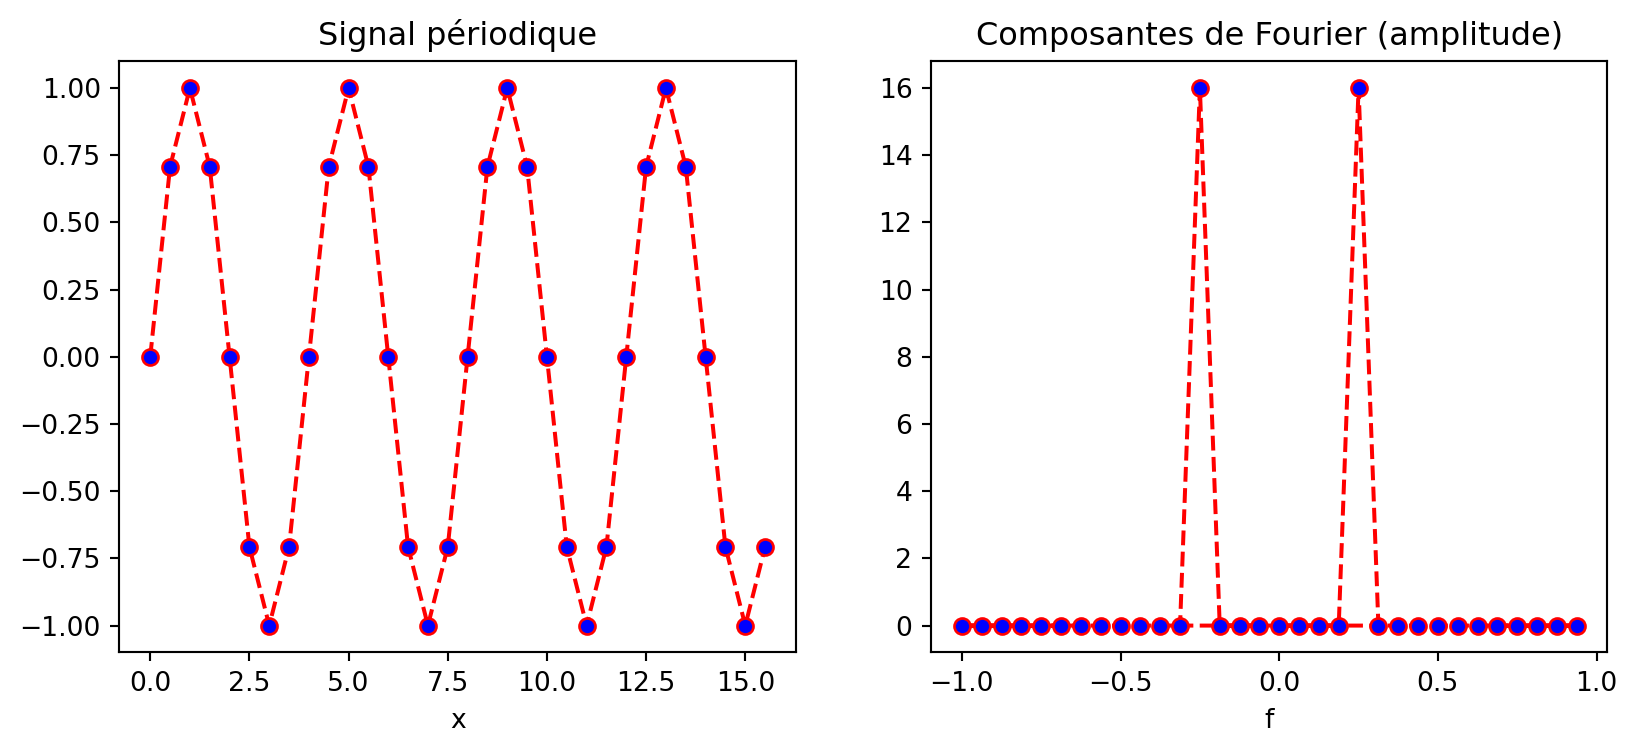
\includegraphics[width=8.52083in,height=3.92708in]{04-TransformationSpatiales_files/figure-html/cell-6-output-1.png}
\caption{}
\end{figure}

\subsubsection{\texorpdfstring{{5.2.2} Filtrage
fréquentielle}{5.2.2 Filtrage fréquentielle}}\label{filtrage-fruxe9quentielle}

Un filtrage fréquentiel consiste à modifier le spectre de Fourier afin
d'éliminer ou de réduire certaines composantes fréquentielles. On peut
distinguer trois grandes catégories de filtres fréquentiels:

\begin{enumerate}
\def\labelenumi{\arabic{enumi}.}
\item
  Les filtres passe-bas qui ne préservent que les basses fréquences
  pour, par exemple, lisser une image.
\item
  Les filtres passe-hauts qui ne préservent que les hautes fréquences
  pour ne préserver que les détails.
\item
  Les filtres passe-bandes qui vont préserver les fréquences dans une
  bande de fréquence particulière.
\end{enumerate}

La librairie \texttt{Scipy} contient différents filtres fréquentielles.
Notez, qu'un filtrage fréquentielle est une simple multiplication de la
réponse du filtre {\textbackslash(F{[}k{]}\textbackslash)} par les
composantes fréquentielles du signal à filtrer
{\textbackslash(X{[}k{]}\textbackslash)}:

\phantomsection\label{eq-fourier-filter}{{\textbackslash{[} X\_f{[}k{]}
= F{[}k{]} \textbackslash times X{[}k{]}
\textbackslash tag\{5.3\}\textbackslash{]}}}

À noter que cette multiplication dans l'espace de Fourier est
équivalente à une opération de convolution dans l'espace originale du
signal {\textbackslash(x\textbackslash)}:

\phantomsection\label{eq-convolve}{{\textbackslash{[} x\_f =
IDFT\^{}\{-1\}{[}F{]}*x \textbackslash tag\{5.4\}\textbackslash{]}}}

\phantomsection\label{9ba87d7d}
\phantomsection\label{cb6}
\begin{Shaded}
\begin{Highlighting}[]
\NormalTok{fig, (ax1, ax2) }\OperatorTok{=}\NormalTok{ plt.subplots(}\DecValTok{1}\NormalTok{, }\DecValTok{2}\NormalTok{, figsize}\OperatorTok{=}\NormalTok{(}\DecValTok{10}\NormalTok{, }\DecValTok{4}\NormalTok{))}
\NormalTok{input\_ }\OperatorTok{=}\NormalTok{ numpy.fft.fft2(img\_rgb.to\_numpy()) }
\NormalTok{result }\OperatorTok{=}\NormalTok{ [ndimage.fourier\_gaussian(input\_[b], sigma}\OperatorTok{=}\DecValTok{4}\NormalTok{) }\ControlFlowTok{for}\NormalTok{ b }\KeywordTok{in} \BuiltInTok{range}\NormalTok{(}\DecValTok{3}\NormalTok{)] }\CommentTok{\# on filtre chaque bande avec un filtre Gaussien}
\NormalTok{result }\OperatorTok{=}\NormalTok{ numpy.fft.ifft2(result)}
\NormalTok{ax1.imshow(img\_rgb.to\_numpy().transpose(}\DecValTok{1}\NormalTok{, }\DecValTok{2}\NormalTok{, }\DecValTok{0}\NormalTok{).astype(}\StringTok{\textquotesingle{}uint8\textquotesingle{}}\NormalTok{))}
\NormalTok{ax1.set\_title(}\StringTok{\textquotesingle{}Originale\textquotesingle{}}\NormalTok{)}
\NormalTok{ax2.imshow(result.real.transpose(}\DecValTok{1}\NormalTok{, }\DecValTok{2}\NormalTok{, }\DecValTok{0}\NormalTok{).astype(}\StringTok{\textquotesingle{}uint8\textquotesingle{}}\NormalTok{))  }\CommentTok{\# La partie imaginaire n\textquotesingle{}est pas utile ici}
\NormalTok{ax2.set\_title(}\StringTok{\textquotesingle{}Filtrage Gaussien\textquotesingle{}}\NormalTok{)}
\NormalTok{plt.show()}
\end{Highlighting}
\end{Shaded}

\begin{figure}
\centering
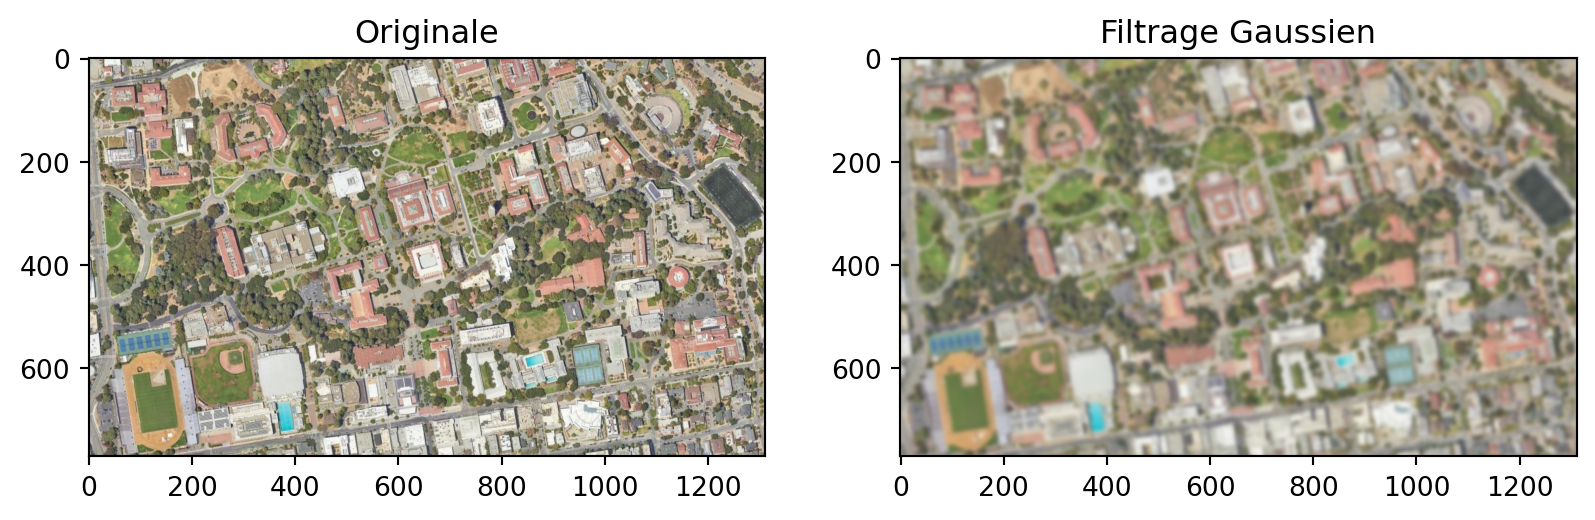
\includegraphics[width=8.3125in,height=2.70833in]{04-TransformationSpatiales_files/figure-html/cell-7-output-1.png}
\caption{}
\end{figure}

\subsubsection{\texorpdfstring{{5.2.3}
L'aliasing}{5.2.3 L'aliasing}}\label{laliasing}

L'aliasing est un problème fréquent en traitement du signal. Il résulte
d'une fréquence d'échantillonnage trop faible par rapport au contenu
fréquentielle du signal. Ceci peut se produire lorsque vous
sous-échantillonner fortement une image avec un facteur de décimation
(par exemple 1 pixel sur 2). En prenant un pixel sur 2, on réduit la
fréquence d'échantillonnage d'un facteur 2 ce qui nous impose de réduire
le contenu fréquentielle de l'image et donc les fréquences maximales de
l'image. L'image présente alors un aspect faussement texturée avec
beaucoup de haute fréquences:

\phantomsection\label{775acc61}
\phantomsection\label{cb7}
\begin{Shaded}
\begin{Highlighting}[]
\NormalTok{fig, axes }\OperatorTok{=}\NormalTok{ plt.subplots(nrows}\OperatorTok{=}\DecValTok{1}\NormalTok{, ncols}\OperatorTok{=}\DecValTok{2}\NormalTok{, figsize}\OperatorTok{=}\NormalTok{(}\DecValTok{10}\NormalTok{, }\DecValTok{4}\NormalTok{))}
\NormalTok{plt.subplot(}\DecValTok{1}\NormalTok{, }\DecValTok{2}\NormalTok{, }\DecValTok{1}\NormalTok{)}
\NormalTok{img\_rgb.astype(}\StringTok{\textquotesingle{}int\textquotesingle{}}\NormalTok{).plot.imshow(rgb}\OperatorTok{=}\StringTok{"band"}\NormalTok{)}
\NormalTok{axes[}\DecValTok{0}\NormalTok{].set\_title(}\StringTok{"Originale"}\NormalTok{)}
\NormalTok{plt.subplot(}\DecValTok{1}\NormalTok{, }\DecValTok{2}\NormalTok{, }\DecValTok{2}\NormalTok{)}
\NormalTok{img\_rgb[:,::}\DecValTok{4}\NormalTok{,::}\DecValTok{4}\NormalTok{].astype(}\StringTok{\textquotesingle{}int\textquotesingle{}}\NormalTok{).plot.imshow(rgb}\OperatorTok{=}\StringTok{"band"}\NormalTok{)}
\NormalTok{axes[}\DecValTok{1}\NormalTok{].set\_title(}\StringTok{"Décimée par un facteur 4"}\NormalTok{)}
\NormalTok{plt.show()}
\end{Highlighting}
\end{Shaded}

\begin{figure}
\centering
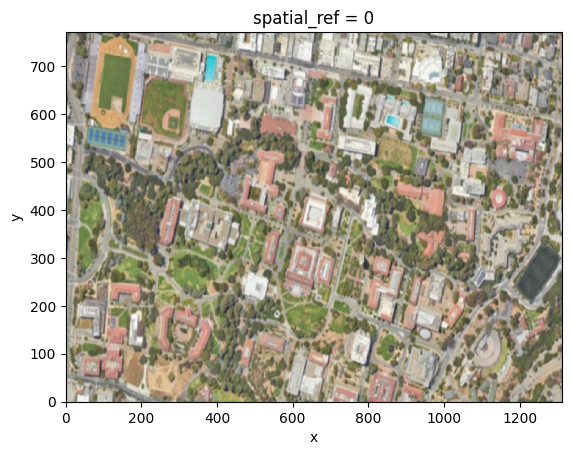
\includegraphics[width=8.5in,height=3.92708in]{04-TransformationSpatiales_files/figure-html/cell-8-output-1.png}
\caption{}
\end{figure}

Une façon de réduire le contenu fréquentiel est de filtrer par un filtre
passe-bas pour réduire les hautes fréquences par exemple avec un filtre
Gaussien:

\phantomsection\label{f7ea15ed}
\phantomsection\label{cb8}
\begin{Shaded}
\begin{Highlighting}[]
\ImportTok{from}\NormalTok{ scipy.ndimage }\ImportTok{import}\NormalTok{ gaussian\_filter}
\NormalTok{q}\OperatorTok{=} \DecValTok{4}
\NormalTok{sigma}\OperatorTok{=}\NormalTok{ q}\OperatorTok{*}\FloatTok{1.1774}\OperatorTok{/}\NormalTok{math.pi}
\NormalTok{arr }\OperatorTok{=}\NormalTok{ xr.DataArray(gaussian\_filter(img\_rgb.to\_numpy(), sigma}\OperatorTok{=}\NormalTok{ (}\DecValTok{0}\NormalTok{,sigma,sigma)), dims}\OperatorTok{=}\NormalTok{(}\StringTok{\textquotesingle{}band\textquotesingle{}}\NormalTok{,}\StringTok{"y"}\NormalTok{, }\StringTok{"x"}\NormalTok{), coords}\OperatorTok{=}\NormalTok{ \{}\StringTok{\textquotesingle{}x\textquotesingle{}}\NormalTok{: img\_rgb.coords[}\StringTok{\textquotesingle{}x\textquotesingle{}}\NormalTok{], }\StringTok{\textquotesingle{}y\textquotesingle{}}\NormalTok{: img\_rgb.coords[}\StringTok{\textquotesingle{}y\textquotesingle{}}\NormalTok{], }\StringTok{\textquotesingle{}spatial\_ref\textquotesingle{}}\NormalTok{: }\DecValTok{0}\NormalTok{\})}

\NormalTok{fig, axes }\OperatorTok{=}\NormalTok{ plt.subplots(nrows}\OperatorTok{=}\DecValTok{1}\NormalTok{, ncols}\OperatorTok{=}\DecValTok{2}\NormalTok{, figsize}\OperatorTok{=}\NormalTok{(}\DecValTok{10}\NormalTok{, }\DecValTok{4}\NormalTok{))}
\NormalTok{plt.subplot(}\DecValTok{1}\NormalTok{, }\DecValTok{2}\NormalTok{, }\DecValTok{1}\NormalTok{)}
\NormalTok{img\_rgb.astype(}\StringTok{\textquotesingle{}int\textquotesingle{}}\NormalTok{).plot.imshow(rgb}\OperatorTok{=}\StringTok{"band"}\NormalTok{)}
\NormalTok{axes[}\DecValTok{0}\NormalTok{].set\_title(}\StringTok{"Originale"}\NormalTok{)}
\NormalTok{plt.subplot(}\DecValTok{1}\NormalTok{, }\DecValTok{2}\NormalTok{, }\DecValTok{2}\NormalTok{)}
\NormalTok{arr[:,::q,::q].astype(}\StringTok{\textquotesingle{}int\textquotesingle{}}\NormalTok{).plot.imshow(rgb}\OperatorTok{=}\StringTok{"band"}\NormalTok{)}
\NormalTok{axes[}\DecValTok{1}\NormalTok{].set\_title(}\StringTok{"Décimée par un facteur 4"}\NormalTok{)}
\NormalTok{plt.show()}
\end{Highlighting}
\end{Shaded}

\begin{figure}
\centering
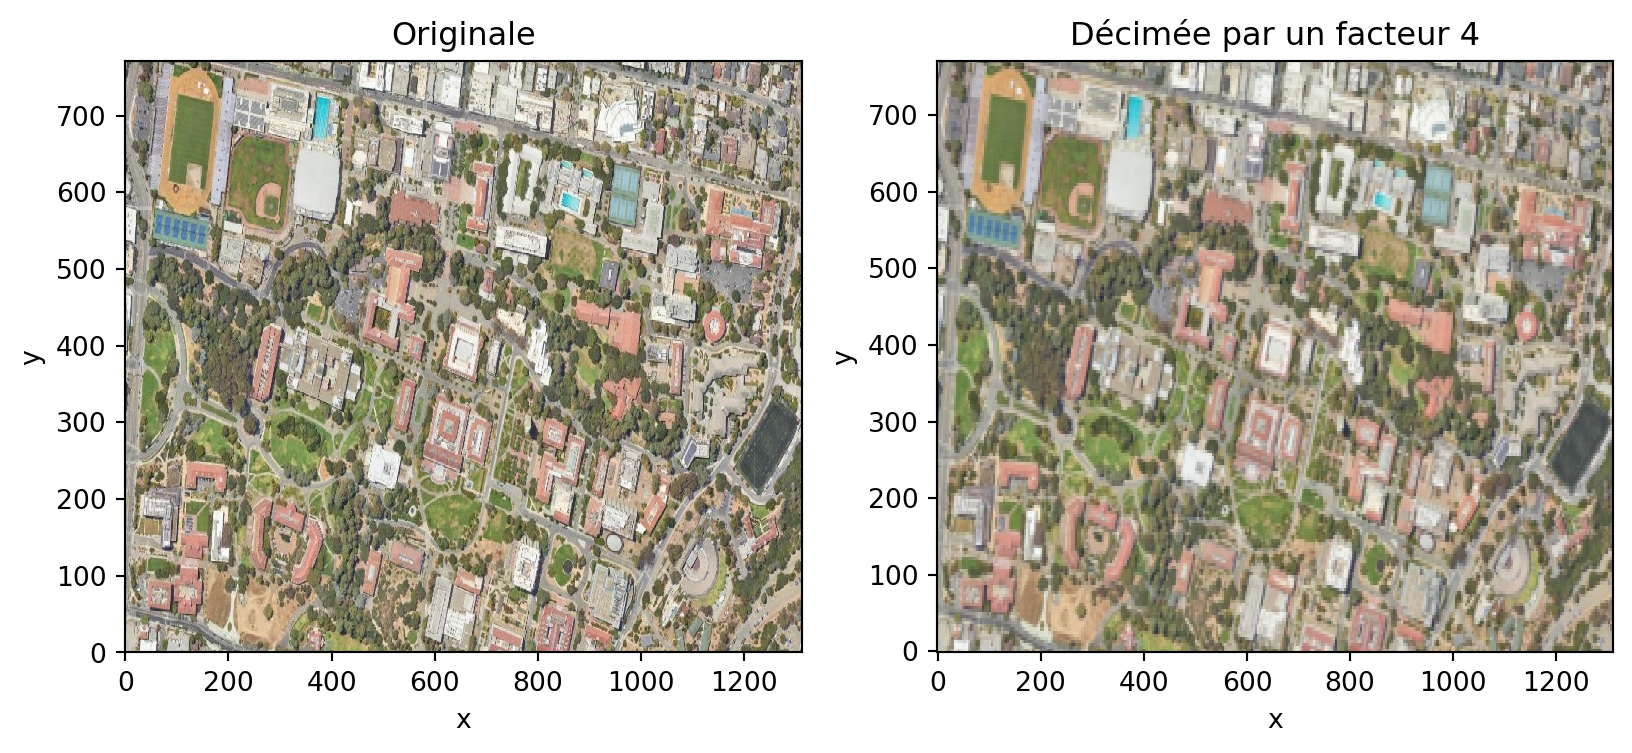
\includegraphics[width=8.5in,height=3.92708in]{04-TransformationSpatiales_files/figure-html/cell-9-output-1.png}
\caption{}
\end{figure}

La fonction
\href{https://docs.scipy.org/doc/scipy/reference/generated/scipy.signal.decimate.html\#scipy.signal.decimate}{\texttt{decimate}}
dans \texttt{scipy.signal} réalise l'opération de décimation
(\emph{downsampling}) en une seule étape:

\phantomsection\label{c68e548a}
\phantomsection\label{cb9}
\begin{Shaded}
\begin{Highlighting}[]
\ImportTok{import}\NormalTok{ xrscipy.signal }\ImportTok{as}\NormalTok{ dsp}

\NormalTok{fig, axes }\OperatorTok{=}\NormalTok{ plt.subplots(nrows}\OperatorTok{=}\DecValTok{1}\NormalTok{, ncols}\OperatorTok{=}\DecValTok{2}\NormalTok{, figsize}\OperatorTok{=}\NormalTok{(}\DecValTok{10}\NormalTok{, }\DecValTok{4}\NormalTok{))}
\NormalTok{plt.subplot(}\DecValTok{1}\NormalTok{, }\DecValTok{2}\NormalTok{, }\DecValTok{1}\NormalTok{)}
\NormalTok{img\_rgb.astype(}\StringTok{\textquotesingle{}int\textquotesingle{}}\NormalTok{).plot.imshow(rgb}\OperatorTok{=}\StringTok{"band"}\NormalTok{)}
\NormalTok{axes[}\DecValTok{0}\NormalTok{].set\_title(}\StringTok{"Originale"}\NormalTok{)}
\NormalTok{plt.subplot(}\DecValTok{1}\NormalTok{, }\DecValTok{2}\NormalTok{, }\DecValTok{2}\NormalTok{)}
\NormalTok{dsp.decimate(img\_rgb, q}\OperatorTok{=}\DecValTok{4}\NormalTok{, dim}\OperatorTok{=}\StringTok{\textquotesingle{}x\textquotesingle{}}\NormalTok{).astype(}\StringTok{\textquotesingle{}int\textquotesingle{}}\NormalTok{).plot.imshow(rgb}\OperatorTok{=}\StringTok{"band"}\NormalTok{)}
\NormalTok{axes[}\DecValTok{1}\NormalTok{].set\_title(}\StringTok{"Décimée par un facteur 4"}\NormalTok{)}
\end{Highlighting}
\end{Shaded}

\begin{verbatim}
Text(0.5, 1.0, 'Décimée par un facteur 4')
\end{verbatim}

\begin{figure}
\centering
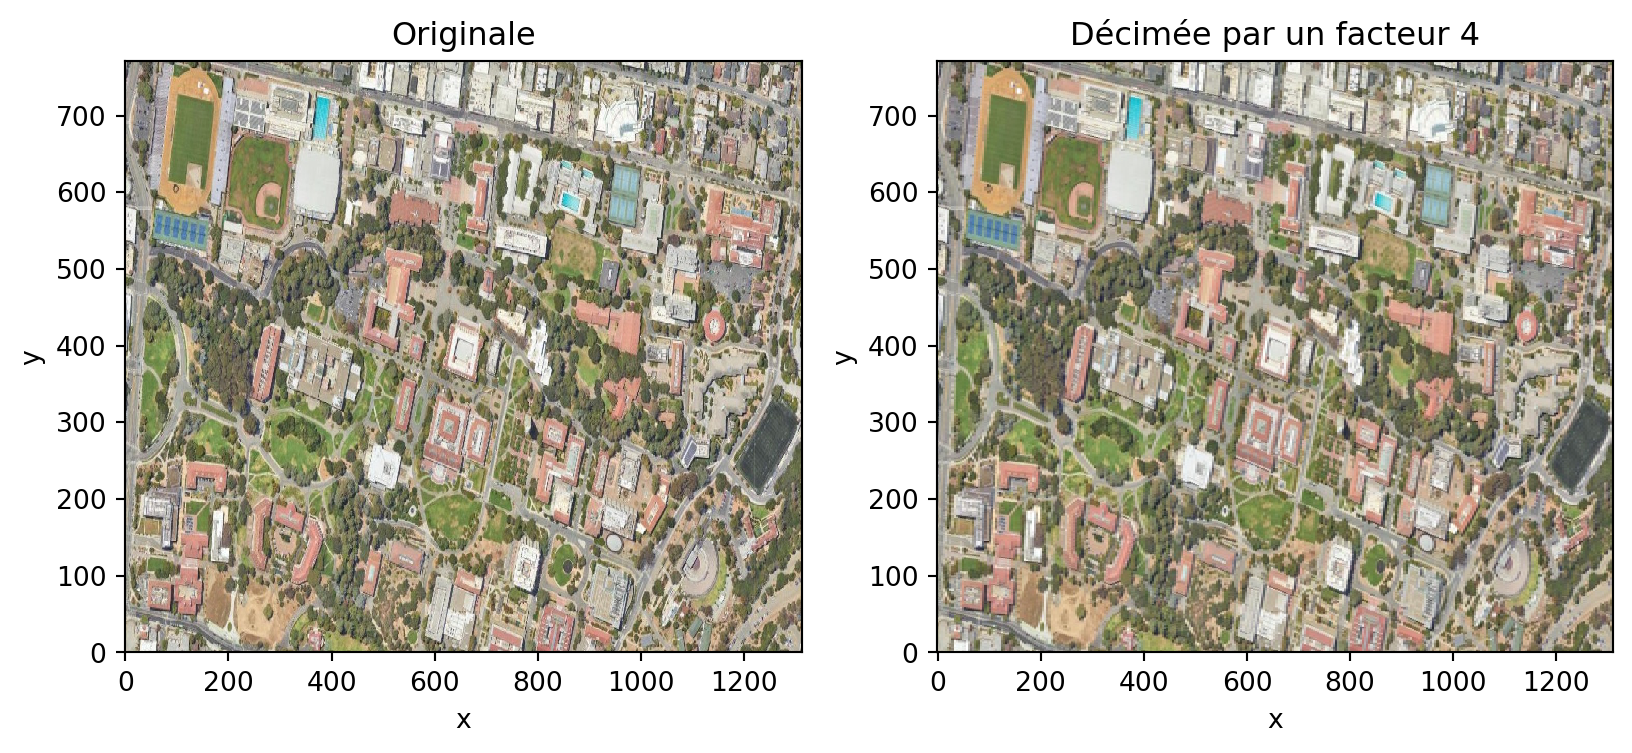
\includegraphics[width=8.5in,height=3.92708in]{04-TransformationSpatiales_files/figure-html/cell-10-output-2.png}
\caption{}
\end{figure}

\subsection{\texorpdfstring{{5.3} Filtrage
d'image}{5.3 Filtrage d'image}}\label{filtrage-dimage}

Le filtrage d'image a plusieurs objectifs en télédétection:

\begin{enumerate}
\def\labelenumi{\arabic{enumi}.}
\item
  La réduction du bruit afin d'améliorer la résolution radiométrique et
  améliorer la lisibilité de l'image.
\item
  Le réhaussement de l'image afin d'améliorer le contraste ou faire
  ressortir les contours.
\item
  La production de nouvelles caractéristiques: c.à.d dériver de
  nouvelles images mettant en valeur certaines informations dans l'image
  comme la texture, les contours, etc.
\end{enumerate}

Il existe de nombreuses méthodes de filtrage dans la littérature, on
peut rassembler ces filtres en quatre grandes catégories:

\begin{enumerate}
\def\labelenumi{\arabic{enumi}.}
\item
  Le filtrage peut-être global ou local, c.à.d prendre en compte toute
  l'image pour filtrer (ex: filtrage par Fourier) ou seulement
  localement avec une fenêtre ou un voisinage local.
\item
  La fonction de filtrage peut-être linéaire ou non linéaire.
\item
  La fonction de filtrage peut être stationnaire ou adaptative
\item
  Le filtrage peut-être mono-échelle ou multi-échelles
\end{enumerate}

La librairie \texttt{Scipy}
(\href{https://docs.scipy.org/doc/scipy/reference/ndimage.html}{Multidimensional
image processing (scipy.ndimage)}) contient une panoplie complète de
filtres.

\subsubsection{\texorpdfstring{{5.3.1} Filtrage linéaire
stationnaire}{5.3.1 Filtrage linéaire stationnaire}}\label{filtrage-linuxe9aire-stationnaire}

Un filtrage linéaire stationnaire consiste à appliquer une même
pondération locale des valeurs des pixels dans une fenêtre glissante. La
taille de cette fenêtre est généralement un chiffre impaire (3,5, etc.)
afin de définir une position centrale et une fenêtre symétrique. La
valeur calculée à partir de tous les pixels dans la fenêtre est alors
attribuée au pixel central.

\emph{}

Note

Mettre une figure ici

Le filtre le plus simple est certainement le filtre moyen qui consiste à
appliquer le même poids uniforme dans la fenêtre glissante. Par exemple
pour un filtre 5x5:

\phantomsection\label{eq-boxfilter}{{\textbackslash{[} F=
\textbackslash frac\{1\}\{25\}\textbackslash left{[}
\textbackslash begin\{array\}\{c\textbar c\textbar c\textbar c\textbar c\}
1 \& 1 \& 1 \& 1 \& 1 \textbackslash\textbackslash{}
\textbackslash hline 1 \& 1 \& 1 \& 1 \& 1
\textbackslash\textbackslash{} \textbackslash hline 1 \& 1 \& 1 \& 1 \&
1 \textbackslash\textbackslash{} \textbackslash hline 1 \& 1 \& 1 \& 1
\& 1 \textbackslash\textbackslash{} \textbackslash hline 1 \& 1 \& 1 \&
1 \& 1 \textbackslash end\{array\} \textbackslash right{]}
\textbackslash tag\{5.5\}\textbackslash{]}}}

En python, on dispose des fonctions \texttt{rolling} et
\texttt{sliding\_window} définis dans la librairie \texttt{numpy}. Par
exemple pour le cas du filtre moyen on peut construire une nouvelle vue
de l'image avec deux nouvelles dimensions \texttt{x\_win} et
\texttt{y\_win}:

\phantomsection\label{3b1b4246}
\phantomsection\label{cb11}
\begin{Shaded}
\begin{Highlighting}[]
\NormalTok{rolling\_win }\OperatorTok{=}\NormalTok{ img\_rgb.rolling(x}\OperatorTok{=}\DecValTok{5}\NormalTok{, y}\OperatorTok{=}\DecValTok{5}\NormalTok{,  min\_periods}\OperatorTok{=} \DecValTok{3}\NormalTok{, center}\OperatorTok{=} \VariableTok{True}\NormalTok{).construct(x}\OperatorTok{=}\StringTok{"x\_win"}\NormalTok{, y}\OperatorTok{=}\StringTok{"y\_win"}\NormalTok{, keep\_attrs}\OperatorTok{=} \VariableTok{True}\NormalTok{)}
\BuiltInTok{print}\NormalTok{(rolling\_win[}\DecValTok{0}\NormalTok{,}\DecValTok{0}\NormalTok{,}\DecValTok{1}\NormalTok{,...])}
\BuiltInTok{print}\NormalTok{(rolling\_win.shape)}
\end{Highlighting}
\end{Shaded}

\begin{verbatim}
<xarray.DataArray (x_win: 5, y_win: 5)> Size: 100B
array([[ nan,  nan,  nan,  nan,  nan],
       [ nan,  nan, 209., 210., 209.],
       [ nan,  nan, 213., 214., 212.],
       [ nan,  nan, 213., 212., 210.],
       [ nan,  nan, 210., 209., 206.]], dtype=float32)
Coordinates:
    band         int64 8B 1
    x            float64 8B 1.5
    y            float64 8B 0.5
    spatial_ref  int64 8B 0
Dimensions without coordinates: x_win, y_win
(3, 771, 1311, 5, 5)
\end{verbatim}

L'avantage de cette approche est qu'il n'y a pas d'utilisation inutile
de la mémoire. Noter les \texttt{nan} sur les bords de l'image car la
fenêtre déborde sur les bordures de l'image. Par la suite un opérateur
moyenne peut être appliqué sur les axes \texttt{x\_win} et
\texttt{y\_win} correspondant aux fenêtres glissantes.

\phantomsection\label{e4e11bbc}
\phantomsection\label{cb13}
\begin{Shaded}
\begin{Highlighting}[]
\NormalTok{filtre\_moyen}\OperatorTok{=}\NormalTok{ rolling\_win.mean(dim}\OperatorTok{=}\NormalTok{ [}\StringTok{\textquotesingle{}x\_win\textquotesingle{}}\NormalTok{, }\StringTok{\textquotesingle{}y\_win\textquotesingle{}}\NormalTok{], skipna}\OperatorTok{=} \VariableTok{True}\NormalTok{)}
\NormalTok{fig, ax }\OperatorTok{=}\NormalTok{ plt.subplots(nrows}\OperatorTok{=}\DecValTok{1}\NormalTok{, ncols}\OperatorTok{=}\DecValTok{1}\NormalTok{, figsize}\OperatorTok{=}\NormalTok{(}\DecValTok{8}\NormalTok{, }\DecValTok{4}\NormalTok{))}
\NormalTok{filtre\_moyen.astype(}\StringTok{\textquotesingle{}int\textquotesingle{}}\NormalTok{).plot.imshow(rgb}\OperatorTok{=}\StringTok{"band"}\NormalTok{)}
\NormalTok{ax.set\_title(}\StringTok{"Filtre moyen 5x5"}\NormalTok{)}
\end{Highlighting}
\end{Shaded}

\begin{verbatim}
Text(0.5, 1.0, 'Filtre moyen 5x5')
\end{verbatim}

\begin{figure}
\centering
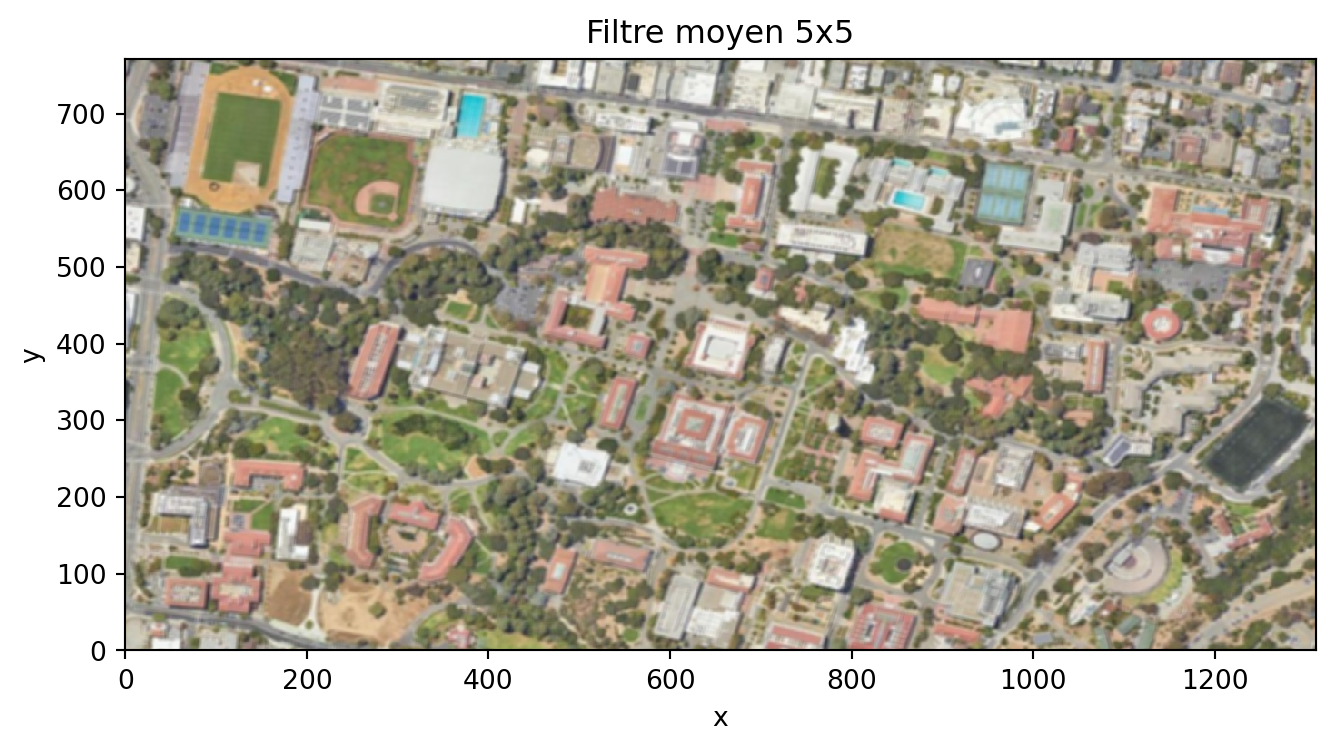
\includegraphics[width=6.94792in,height=3.91667in]{04-TransformationSpatiales_files/figure-html/cell-12-output-2.png}
\caption{}
\end{figure}

Lorsque la taille {\textbackslash(W\textbackslash)} de la fenêtre
devient trop grande, il est préférable d'utiliser une convolution dans
le domaine fréquentielle. La fonction \texttt{fftconvolve} de la
librairie \texttt{scipy.signal} permet de faire cela:

\phantomsection\label{ffbbf43e}
\phantomsection\label{cb15}
\begin{Shaded}
\begin{Highlighting}[]
\NormalTok{kernel }\OperatorTok{=}\NormalTok{ np.outer(signal.windows.gaussian(}\DecValTok{70}\NormalTok{, }\DecValTok{8}\NormalTok{),}
\NormalTok{                  signal.windows.gaussian(}\DecValTok{70}\NormalTok{, }\DecValTok{8}\NormalTok{))}
\NormalTok{blurred }\OperatorTok{=}\NormalTok{ signal.fftconvolve(img\_rgb, kernel, mode}\OperatorTok{=}\StringTok{\textquotesingle{}same\textquotesingle{}}\NormalTok{)}
\end{Highlighting}
\end{Shaded}

\emph{}

Note

Filtre de Sobel, filtre Prewitt

\paragraph{\texorpdfstring{{5.3.1.1} Filtrage par
convolution}{5.3.1.1 Filtrage par convolution}}\label{filtrage-par-convolution}

La façon la plus efficace d'appliquer un filtre linéaire est d'appliquer
une convolution. La convolution est généralement très efficace car elle
est peut être calculée dans le domaine fréquentielle. Prenons l'exemple
du filtre de Scharr {(\href{references.html\#ref-Scharr1999}{Jahne et S.
1999})}, ce filtre permet de détecter les contours horizontaux et
verticaux:

\phantomsection\label{eq-scharr-filter}{{\textbackslash{[} F=
\textbackslash left{[} \textbackslash begin\{array\}\{ccc\} -3-3j \&
0-10j \& +3-3j \textbackslash\textbackslash{} -10+0j \& 0+0j \& +10+0j
\textbackslash\textbackslash{} -3+3j \& 0+10j \& +3+3j
\textbackslash end\{array\} \textbackslash right{]}
\textbackslash tag\{5.6\}\textbackslash{]}}}

Remarquez l'utilisation de chiffres complexes afin de passer deux
filtres différents sur la partie réelle et imaginaire.

\phantomsection\label{8a8cbdf9}
\phantomsection\label{cb16}
\begin{Shaded}
\begin{Highlighting}[]
\NormalTok{scharr }\OperatorTok{=}\NormalTok{ np.array([[ }\OperatorTok{{-}}\DecValTok{3}\OperatorTok{{-}}\OtherTok{3j}\NormalTok{, }\DecValTok{0}\OperatorTok{{-}}\OtherTok{10j}\NormalTok{,  }\OperatorTok{+}\DecValTok{3} \OperatorTok{{-}}\OtherTok{3j}\NormalTok{],}
\NormalTok{                   [}\OperatorTok{{-}}\DecValTok{10}\OperatorTok{+}\OtherTok{0j}\NormalTok{, }\DecValTok{0}\OperatorTok{+} \OtherTok{0j}\NormalTok{, }\OperatorTok{+}\DecValTok{10} \OperatorTok{+}\OtherTok{0j}\NormalTok{],}
\NormalTok{                   [ }\OperatorTok{{-}}\DecValTok{3}\OperatorTok{+}\OtherTok{3j}\NormalTok{, }\DecValTok{0}\OperatorTok{+}\OtherTok{10j}\NormalTok{,  }\OperatorTok{+}\DecValTok{3} \OperatorTok{+}\OtherTok{3j}\NormalTok{]]) }\CommentTok{\# Gx + j*Gy}
\BuiltInTok{print}\NormalTok{(img\_rgb.isel(band}\OperatorTok{=}\DecValTok{0}\NormalTok{).shape)}
\NormalTok{grad }\OperatorTok{=}\NormalTok{ signal.convolve2d(img\_rgb.isel(band}\OperatorTok{=}\DecValTok{0}\NormalTok{), scharr, boundary}\OperatorTok{=}\StringTok{\textquotesingle{}symm\textquotesingle{}}\NormalTok{, mode}\OperatorTok{=}\StringTok{\textquotesingle{}same\textquotesingle{}}\NormalTok{)}
\CommentTok{\# on reconstruit un xarray à partir du résultat:}
\NormalTok{arr }\OperatorTok{=}\NormalTok{ xr.DataArray(np.}\BuiltInTok{abs}\NormalTok{(grad), dims}\OperatorTok{=}\NormalTok{(}\StringTok{"y"}\NormalTok{, }\StringTok{"x"}\NormalTok{), coords}\OperatorTok{=}\NormalTok{ \{}\StringTok{\textquotesingle{}x\textquotesingle{}}\NormalTok{: img\_rgb.coords[}\StringTok{\textquotesingle{}x\textquotesingle{}}\NormalTok{], }\StringTok{\textquotesingle{}y\textquotesingle{}}\NormalTok{: img\_rgb.coords[}\StringTok{\textquotesingle{}y\textquotesingle{}}\NormalTok{], }\StringTok{\textquotesingle{}spatial\_ref\textquotesingle{}}\NormalTok{: }\DecValTok{0}\NormalTok{\})}
\BuiltInTok{print}\NormalTok{(arr)}
\NormalTok{fig, ax }\OperatorTok{=}\NormalTok{ plt.subplots(nrows}\OperatorTok{=}\DecValTok{1}\NormalTok{, ncols}\OperatorTok{=}\DecValTok{1}\NormalTok{, figsize}\OperatorTok{=}\NormalTok{(}\DecValTok{8}\NormalTok{, }\DecValTok{4}\NormalTok{))}
\NormalTok{arr.plot.imshow()}
\NormalTok{ax.set\_title(}\StringTok{"Amplitude du filtre de Scharr"}\NormalTok{)}
\end{Highlighting}
\end{Shaded}

\begin{verbatim}
(771, 1311)
<xarray.DataArray (y: 771, x: 1311)> Size: 8MB
array([[  65.96969001,   58.85575588,   54.91812087, ..., 1474.        ,
        1037.01205393,  389.99487176],
       [  61.07372594,   39.8246155 ,   89.18520057, ..., 1763.79647352,
         864.92543031,  270.20362692],
       [  98.48857802,  112.44554237,  168.10710871, ..., 2110.61365484,
         870.36658943,  204.40156555],
       ...,
       [ 143.17821063,  597.00753764, 2479.42977315, ...,  216.00925906,
         248.33847869,  200.89798406],
       [ 106.07544485,  393.67245268, 2188.78824924, ...,  124.96399481,
         159.90622252,  346.34087255],
       [  41.59326869,  229.05894438, 1845.1216762 , ...,  175.16278143,
          33.37663854,  414.3911196 ]])
Coordinates:
  * x            (x) float64 10kB 0.5 1.5 2.5 ... 1.308e+03 1.31e+03 1.31e+03
  * y            (y) float64 6kB 0.5 1.5 2.5 3.5 4.5 ... 767.5 768.5 769.5 770.5
    spatial_ref  int64 8B 0
\end{verbatim}

\begin{verbatim}
Text(0.5, 1.0, 'Amplitude du filtre de Scharr')
\end{verbatim}

\begin{figure}
\centering
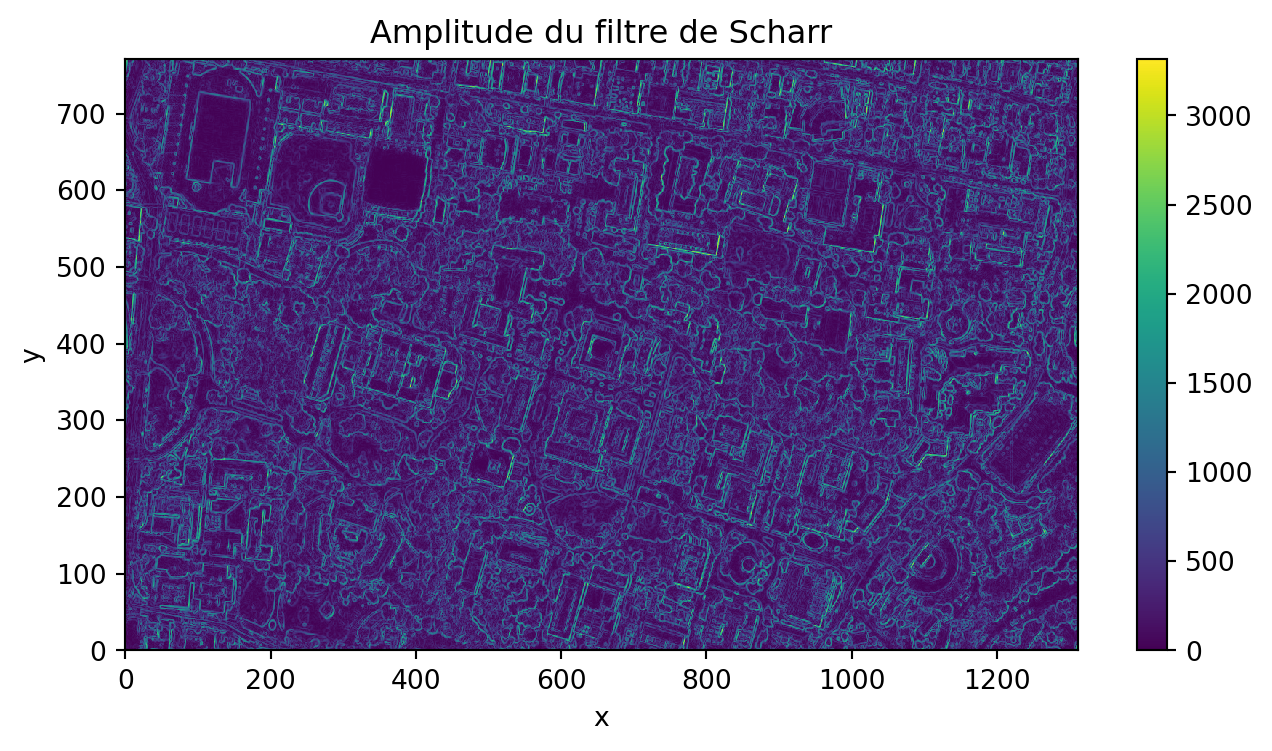
\includegraphics[width=6.625in,height=3.91667in]{04-TransformationSpatiales_files/figure-html/cell-14-output-3.png}
\caption{}
\end{figure}

\emph{}

Gestion des bordures

L'application de filtres à l'intérieur de fenêtres glissantes implique
de gérer les bords de l'image car la fenêtre de traitement va
nécessairement déborder de quelques pixels en dehors de l'image
(généralement la moitié de la fenêtre déborde). On peut soit décider
d'ignorer les valeurs en dehors de l'image en imposant une valeur
\texttt{nan}, prolonger l'image de quelques lignes et colonnes avec des
valeurs mirroirs ou constantes.

\paragraph{\texorpdfstring{{5.3.1.2} Filtrage par une couche
convolutionnelle}{5.3.1.2 Filtrage par une couche convolutionnelle}}\label{filtrage-par-une-couche-convolutionnelle}

\emph{}

Installation de Pytorch

Cette section nécessite la librairie Pytorch avec un GPU et ne
fonctionnera que sur Colab. On peut quand même installer une version
locale CPU de pytorch: \texttt{pip\ install\ -qU\ torch==2.4.0+cpu}

Une couche convolutionnelle est simplement un ensemble de filtres
appliqués sur la donnée d'entrée. Ce type de filtrage est à la base des
réseaux dits convolutionnels qui seront abordés dans le tome 2. On peut
ici imposer les mêmes filtres de gradient dans la couche
convolutionnelle:

\phantomsection\label{e4417b87}
\phantomsection\label{cb19}
\begin{Shaded}
\begin{Highlighting}[]
\ImportTok{import}\NormalTok{ torch}
\ImportTok{import}\NormalTok{ torch.nn }\ImportTok{as}\NormalTok{ nn}
\ImportTok{import}\NormalTok{ numpy }\ImportTok{as}\NormalTok{ np}
\ImportTok{import}\NormalTok{ matplotlib.pyplot }\ImportTok{as}\NormalTok{ plt}
\NormalTok{normalized\_img}\OperatorTok{=}\NormalTok{ torch.tensor(img\_rgb.to\_numpy())}
\NormalTok{nchannels}\OperatorTok{=}\NormalTok{ normalized\_img.size()[}\DecValTok{0}\NormalTok{] }\CommentTok{\# nombre de canaux de l\textquotesingle{}image}

\CommentTok{\# On forme une couche convolutionnelle}
\NormalTok{conv\_layer }\OperatorTok{=}\NormalTok{ nn.Conv2d(in\_channels}\OperatorTok{=}\NormalTok{ nchannels, out\_channels}\OperatorTok{=}\DecValTok{2}\NormalTok{, kernel\_size}\OperatorTok{=}\DecValTok{3}\NormalTok{, padding}\OperatorTok{=}\DecValTok{1}\NormalTok{, stride}\OperatorTok{=}\DecValTok{1}\NormalTok{, dilation}\OperatorTok{=} \DecValTok{1}\NormalTok{)}

\CommentTok{\# Filtre de Sobel}
\NormalTok{sobel\_x }\OperatorTok{=}\NormalTok{ np.array([[}\OperatorTok{{-}}\DecValTok{3}\NormalTok{, }\DecValTok{0}\NormalTok{, }\DecValTok{3}\NormalTok{], [}\OperatorTok{{-}}\DecValTok{10}\NormalTok{, }\DecValTok{0}\NormalTok{, }\DecValTok{10}\NormalTok{], [}\OperatorTok{{-}}\DecValTok{3}\NormalTok{, }\DecValTok{0}\NormalTok{, }\DecValTok{3}\NormalTok{]])}
\NormalTok{sobel\_y }\OperatorTok{=}\NormalTok{ np.array([[}\OperatorTok{{-}}\DecValTok{3}\NormalTok{, }\OperatorTok{{-}}\DecValTok{10}\NormalTok{, }\OperatorTok{{-}}\DecValTok{3}\NormalTok{], [}\DecValTok{0}\NormalTok{, }\DecValTok{0}\NormalTok{, }\DecValTok{0}\NormalTok{], [}\DecValTok{3}\NormalTok{, }\DecValTok{10}\NormalTok{, }\DecValTok{3}\NormalTok{]])}
\CommentTok{\# Le filtre (kernel) est formé de deux filtres}
\NormalTok{kernel }\OperatorTok{=}\NormalTok{ np.stack([sobel\_x, sobel\_y])}
\NormalTok{kernel }\OperatorTok{=}\NormalTok{ kernel.reshape(}\DecValTok{2}\NormalTok{, }\DecValTok{1}\NormalTok{, }\DecValTok{3}\NormalTok{, }\DecValTok{3}\NormalTok{)}
\CommentTok{\# On répète le filtre pour chaque bande}
\NormalTok{kernel }\OperatorTok{=}\NormalTok{ np.tile(kernel,(}\DecValTok{1}\NormalTok{,nchannels,}\DecValTok{1}\NormalTok{,}\DecValTok{1}\NormalTok{))}
\BuiltInTok{print}\NormalTok{(kernel.shape)}
\NormalTok{kernel }\OperatorTok{=}\NormalTok{ torch.as\_tensor(kernel,dtype}\OperatorTok{=}\NormalTok{torch.float32)}
\NormalTok{conv\_layer.weight }\OperatorTok{=}\NormalTok{ nn.Parameter(kernel)}
\NormalTok{conv\_layer.bias }\OperatorTok{=}\NormalTok{ nn.Parameter(torch.zeros(}\DecValTok{2}\NormalTok{,))}

\BuiltInTok{input}\OperatorTok{=}\NormalTok{ normalized\_img.unsqueeze(}\DecValTok{0}\NormalTok{) }\CommentTok{\# il faut ajouter une dimension pour le nombre d\textquotesingle{}échantillons}
\BuiltInTok{print}\NormalTok{(}\BuiltInTok{input}\NormalTok{.shape)}
\CommentTok{\# Visualize the filters}
\NormalTok{fig, axs }\OperatorTok{=}\NormalTok{ plt.subplots(}\DecValTok{1}\NormalTok{, }\DecValTok{2}\NormalTok{, figsize}\OperatorTok{=}\NormalTok{(}\DecValTok{8}\NormalTok{, }\DecValTok{5}\NormalTok{))}
\ControlFlowTok{for}\NormalTok{ i }\KeywordTok{in} \BuiltInTok{range}\NormalTok{(}\DecValTok{2}\NormalTok{):}
\NormalTok{    axs[i].imshow(conv\_layer.weight.data.numpy()[i, }\DecValTok{0}\NormalTok{])}
\NormalTok{    axs[i].set\_title(}\SpecialStringTok{f\textquotesingle{}Filtre }\SpecialCharTok{\{}\NormalTok{i}\OperatorTok{+}\DecValTok{1}\SpecialCharTok{\}}\SpecialStringTok{\textquotesingle{}}\NormalTok{)}
\NormalTok{plt.show()}
\end{Highlighting}
\end{Shaded}

\begin{verbatim}
(2, 3, 3, 3)
torch.Size([1, 3, 771, 1311])
\end{verbatim}

\begin{figure}
\centering
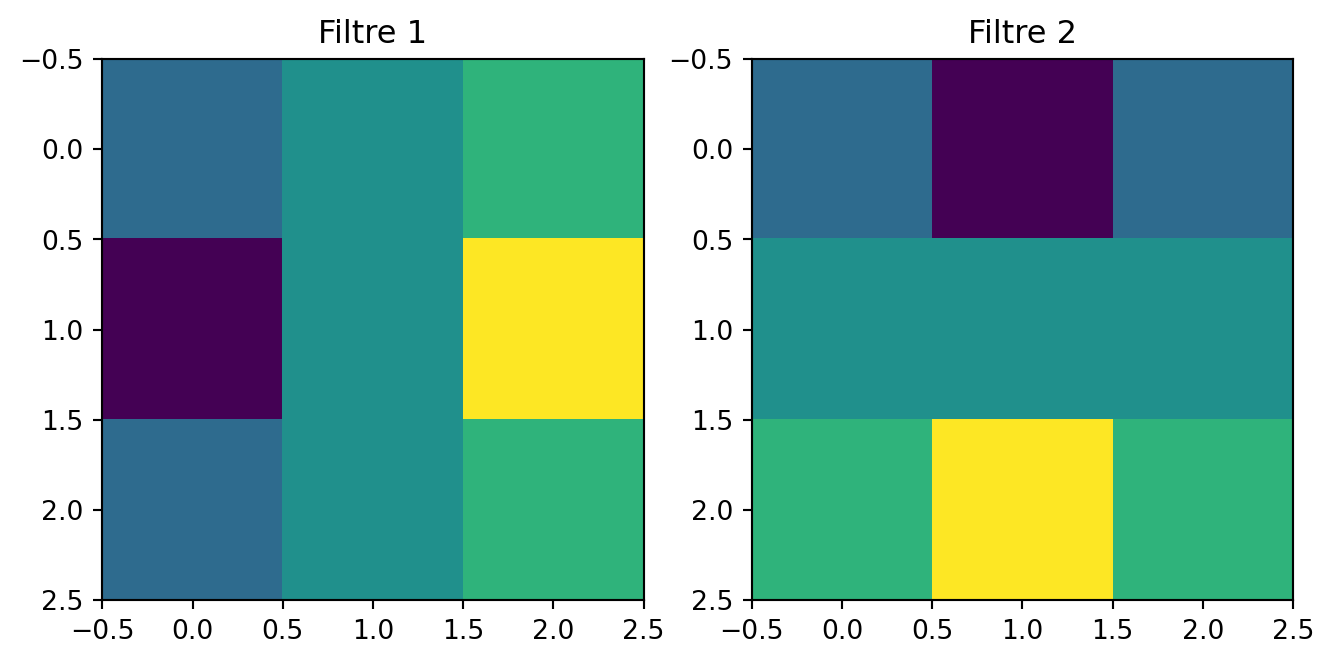
\includegraphics[width=6.94792in,height=3.45833in]{04-TransformationSpatiales_files/figure-html/cell-15-output-2.png}
\caption{}
\end{figure}

Le résultat est alors calculé sur GPU (si disponible):

\phantomsection\label{29c671f0}
\phantomsection\label{cb21}
\begin{Shaded}
\begin{Highlighting}[]
\ImportTok{import}\NormalTok{ torch}
\ImportTok{import}\NormalTok{ matplotlib.pyplot }\ImportTok{as}\NormalTok{ plt}

\NormalTok{output }\OperatorTok{=}\NormalTok{ conv\_layer(}\BuiltInTok{input}\NormalTok{)}
\BuiltInTok{print}\NormalTok{(}\SpecialStringTok{f\textquotesingle{}Image (BxCxHxW): }\SpecialCharTok{\{}\BuiltInTok{input}\SpecialCharTok{.}\NormalTok{shape}\SpecialCharTok{\}}\SpecialStringTok{\textquotesingle{}}\NormalTok{)}
\BuiltInTok{print}\NormalTok{(}\SpecialStringTok{f\textquotesingle{}Sortie (BxFxHxW): }\SpecialCharTok{\{}\NormalTok{output}\SpecialCharTok{.}\NormalTok{shape}\SpecialCharTok{\}}\SpecialStringTok{\textquotesingle{}}\NormalTok{)}

\NormalTok{fig, axs }\OperatorTok{=}\NormalTok{ plt.subplots(}\DecValTok{1}\NormalTok{, }\DecValTok{2}\NormalTok{, figsize}\OperatorTok{=}\NormalTok{(}\DecValTok{20}\NormalTok{, }\DecValTok{5}\NormalTok{))}
\ControlFlowTok{for}\NormalTok{ i }\KeywordTok{in} \BuiltInTok{range}\NormalTok{(}\DecValTok{2}\NormalTok{):}
\NormalTok{    axs[i].imshow(output.detach().data.numpy()[}\DecValTok{0}\NormalTok{,i], vmin}\OperatorTok{={-}}\DecValTok{5000}\NormalTok{, vmax}\OperatorTok{=}\DecValTok{5000}\NormalTok{, cmap}\OperatorTok{=} \StringTok{\textquotesingle{}gray\textquotesingle{}}\NormalTok{)}
\NormalTok{    axs[i].set\_title(}\SpecialStringTok{f\textquotesingle{}Filtrage }\SpecialCharTok{\{}\NormalTok{i}\OperatorTok{+}\DecValTok{1}\SpecialCharTok{\}}\SpecialStringTok{\textquotesingle{}}\NormalTok{)}
\NormalTok{plt.show()}
\end{Highlighting}
\end{Shaded}

\begin{verbatim}
Image (BxCxHxW): torch.Size([1, 3, 771, 1311])
Sortie (BxFxHxW): torch.Size([1, 2, 771, 1311])
\end{verbatim}

\begin{figure}
\centering
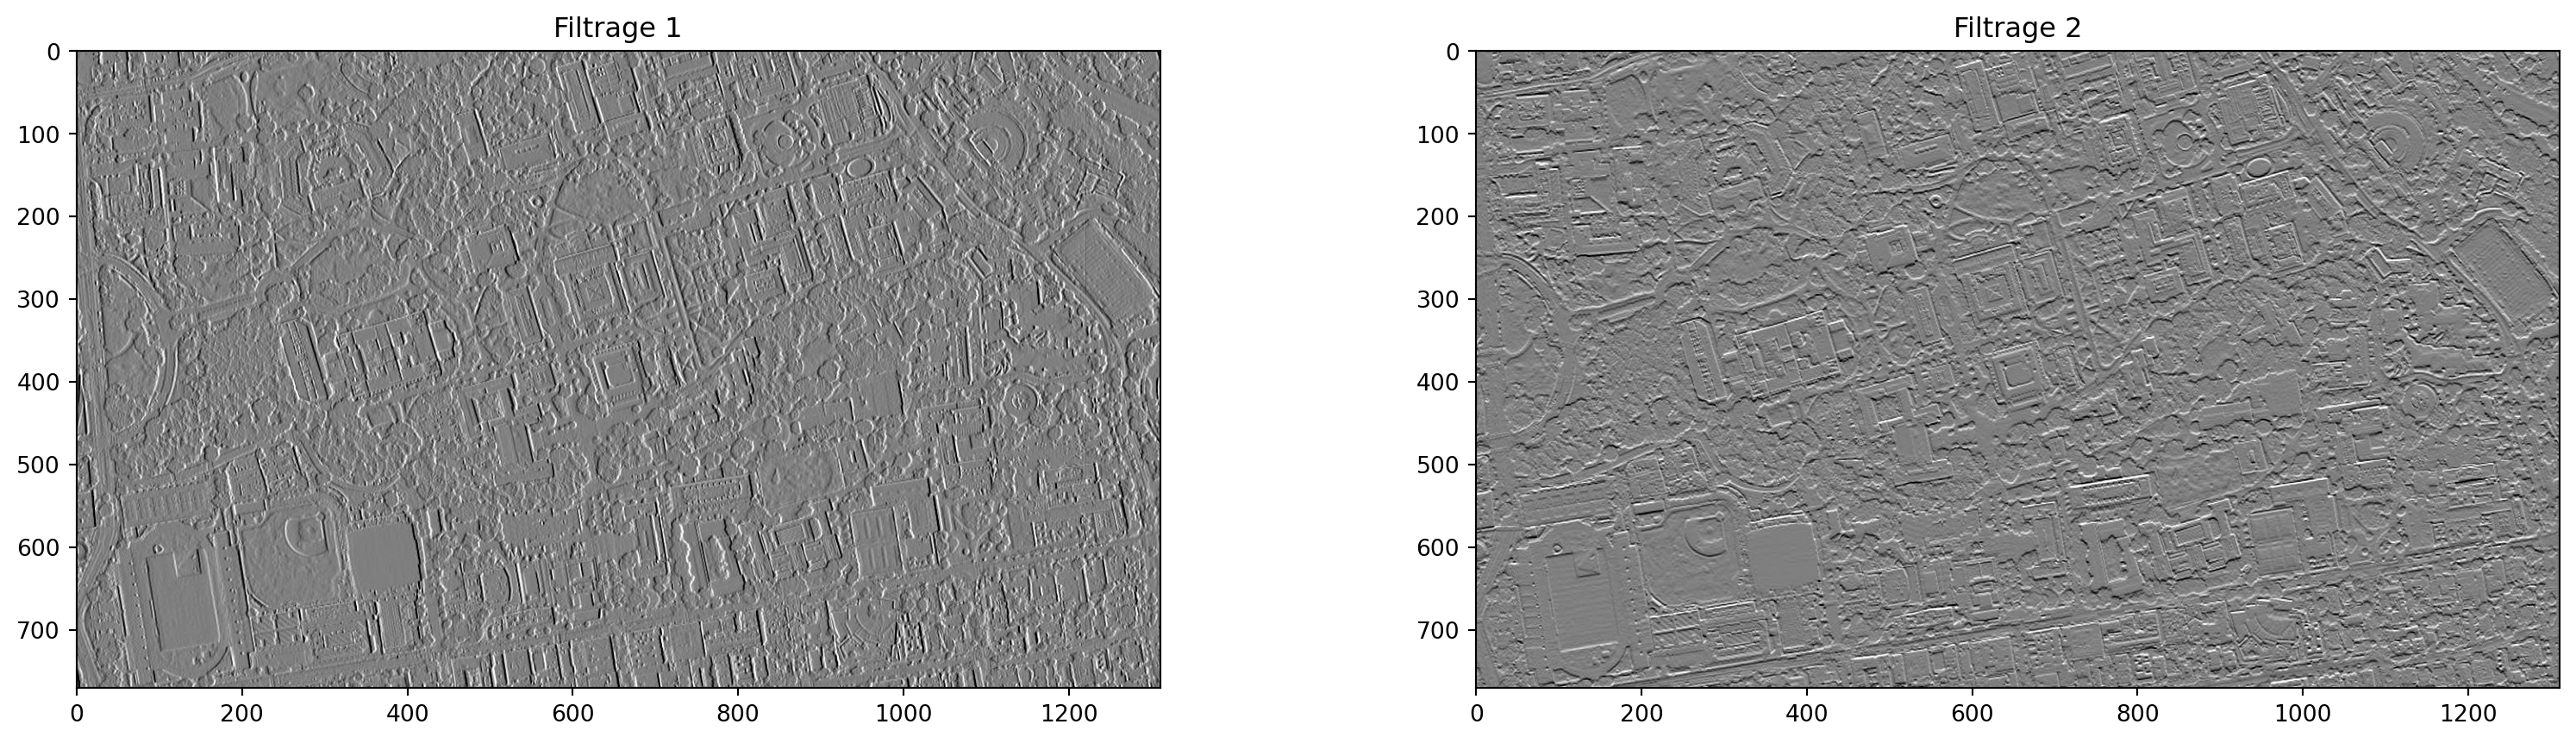
\includegraphics[width=15.5625in,height=4.48958in]{04-TransformationSpatiales_files/figure-html/cell-16-output-2.png}
\caption{}
\end{figure}

\subsubsection{\texorpdfstring{{5.3.2} Filtrage
adaptatif}{5.3.2 Filtrage adaptatif}}\label{filtrage-adaptatif}

Les filtrages adaptatifs consistent à appliquer un traitement en
fonction du contenu local d'une image. Le filtre n'est alors plus
stationnaire et sa réponse peut varier en fonction du contenu local. Ce
type de filtre est très utilisé pour filtrer les images SAR (Synthetic
Aperture Radar) qui sont dégradées par un bruit multiplicatif que l'on
appelle \emph{speckle}. On peut voir un exemple d'une image Sentinel-1
(bande HH) sur la région de Montréal, remarquée que l'image est affichée
en dB en appliquant la fonction \texttt{log10}.

\phantomsection\label{a5a08269}
\phantomsection\label{cb23}
\begin{Shaded}
\begin{Highlighting}[]
\BuiltInTok{print}\NormalTok{(img\_SAR.rio.resolution())}
\BuiltInTok{print}\NormalTok{(img\_SAR.rio.crs)}
\NormalTok{fig, axs }\OperatorTok{=}\NormalTok{ plt.subplots(}\DecValTok{1}\NormalTok{, }\DecValTok{1}\NormalTok{, figsize}\OperatorTok{=}\NormalTok{(}\DecValTok{6}\NormalTok{, }\DecValTok{4}\NormalTok{))}
\NormalTok{xr.ufuncs.log10(img\_SAR.sel(band}\OperatorTok{=}\DecValTok{1}\NormalTok{).drop(}\StringTok{"band"}\NormalTok{)).plot()}
\NormalTok{axs.set\_title(}\StringTok{"Image SAR Sentinel{-}1 (dB)"}\NormalTok{)}
\end{Highlighting}
\end{Shaded}

\begin{verbatim}
(0.00029254428869762705, -0.000287092818453516)
EPSG:4326
\end{verbatim}

\begin{verbatim}
Text(0.5, 1.0, 'Image SAR Sentinel-1 (dB)')
\end{verbatim}

\begin{figure}
\centering
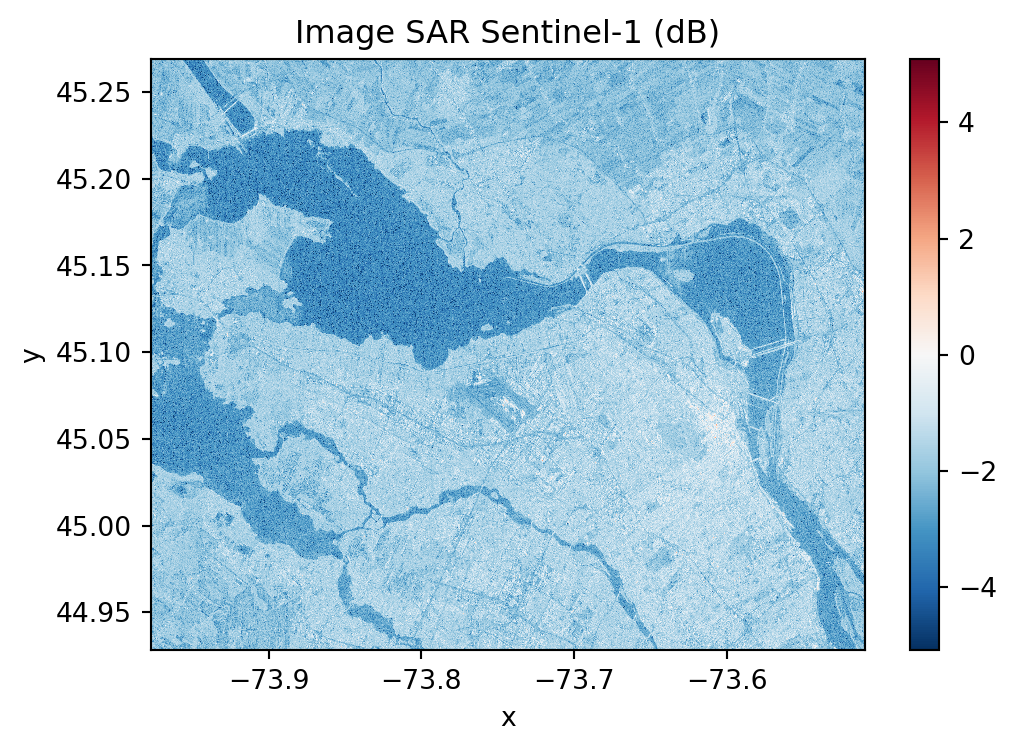
\includegraphics[width=5.29167in,height=3.91667in]{04-TransformationSpatiales_files/figure-html/cell-17-output-3.png}
\caption{}
\end{figure}

Un des filtres les plus simples pour réduire le bruit est d'appliquer un
filtre moyenne, par exemple un {\textbackslash(5 \textbackslash times
5\textbackslash)} ci dessous:

\phantomsection\label{ff1753e5}
\phantomsection\label{cb26}
\begin{Shaded}
\begin{Highlighting}[]
\NormalTok{rolling\_win }\OperatorTok{=}\NormalTok{ img\_SAR.sel(band}\OperatorTok{=}\DecValTok{2}\NormalTok{).rolling(x}\OperatorTok{=}\DecValTok{5}\NormalTok{, y}\OperatorTok{=}\DecValTok{5}\NormalTok{,  min\_periods}\OperatorTok{=} \DecValTok{3}\NormalTok{, center}\OperatorTok{=} \VariableTok{True}\NormalTok{).construct(x}\OperatorTok{=}\StringTok{"x\_win"}\NormalTok{, y}\OperatorTok{=}\StringTok{"y\_win"}\NormalTok{, keep\_attrs}\OperatorTok{=} \VariableTok{True}\NormalTok{)}
\NormalTok{filtre\_moyen}\OperatorTok{=}\NormalTok{ rolling\_win.mean(dim}\OperatorTok{=}\NormalTok{ [}\StringTok{\textquotesingle{}x\_win\textquotesingle{}}\NormalTok{, }\StringTok{\textquotesingle{}y\_win\textquotesingle{}}\NormalTok{], skipna}\OperatorTok{=} \VariableTok{True}\NormalTok{)}
\NormalTok{fig, axs }\OperatorTok{=}\NormalTok{ plt.subplots(}\DecValTok{1}\NormalTok{, }\DecValTok{1}\NormalTok{, figsize}\OperatorTok{=}\NormalTok{(}\DecValTok{6}\NormalTok{, }\DecValTok{4}\NormalTok{))}
\NormalTok{xr.ufuncs.log10(filtre\_moyen).plot.imshow()}
\NormalTok{axs.set\_title(}\StringTok{"Filtrage moyen 5x5 (dB)"}\NormalTok{)}
\end{Highlighting}
\end{Shaded}

\begin{verbatim}
Text(0.5, 1.0, 'Filtrage moyen 5x5 (dB)')
\end{verbatim}

\begin{figure}
\centering
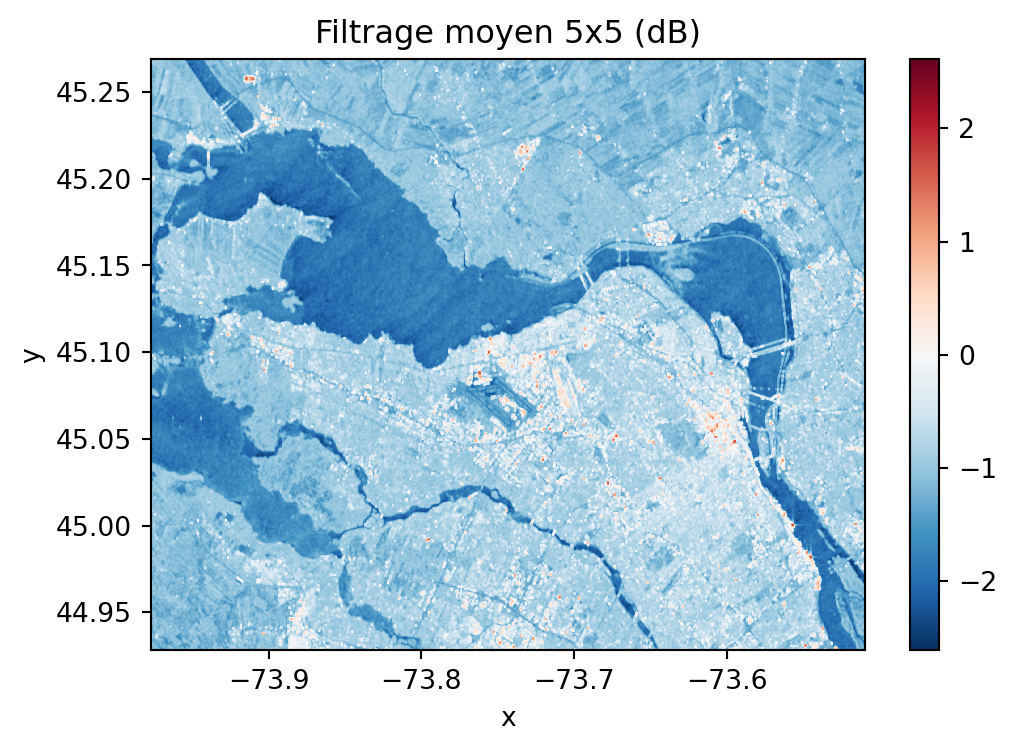
\includegraphics[width=5.29167in,height=3.91667in]{04-TransformationSpatiales_files/figure-html/cell-18-output-2.png}
\caption{}
\end{figure}

Au lieu d'appliquer un filtre moyen de manière indiscriminée, le filtre
de Lee {(\href{references.html\#ref-Lee-1986}{Lee 1986})} applique une
pondération en fonction du contenu local de l'image
{\textbackslash(I\textbackslash)} dans sa forme la plus simple:

\phantomsection\label{eq-lee-filter}{{\textbackslash{[}
\textbackslash begin\{aligned\} I\_F \& = I\_M + K \textbackslash times
(I - I\_M) \textbackslash\textbackslash{} K \& =
\textbackslash frac\{\textbackslash sigma\^{}2\_I\}\{\textbackslash sigma\^{}2\_I
+ \textbackslash sigma\^{}2\_\{bruit\}\} \textbackslash end\{aligned\}
\textbackslash tag\{5.7\}\textbackslash{]}}}

Ainsi si la variance locale est élevée {\textbackslash(K\textbackslash)}
s'approche de {\textbackslash(1\textbackslash)} préservant ainsi les
détails de l'image {\textbackslash(I\textbackslash)} sinon l'image
moyenne {\textbackslash(I\_M\textbackslash)} est appliquée.

\phantomsection\label{59c62e6c}
\phantomsection\label{cb28}
\begin{Shaded}
\begin{Highlighting}[]
\NormalTok{rolling\_win }\OperatorTok{=}\NormalTok{ img\_SAR.sel(band}\OperatorTok{=}\DecValTok{2}\NormalTok{).rolling(x}\OperatorTok{=}\DecValTok{5}\NormalTok{, y}\OperatorTok{=}\DecValTok{5}\NormalTok{,  min\_periods}\OperatorTok{=} \DecValTok{3}\NormalTok{, center}\OperatorTok{=} \VariableTok{True}\NormalTok{).construct(x}\OperatorTok{=}\StringTok{"x\_win"}\NormalTok{, y}\OperatorTok{=}\StringTok{"y\_win"}\NormalTok{, keep\_attrs}\OperatorTok{=} \VariableTok{True}\NormalTok{)}
\NormalTok{filtre\_moyen}\OperatorTok{=}\NormalTok{ rolling\_win.mean(dim}\OperatorTok{=}\NormalTok{ [}\StringTok{\textquotesingle{}x\_win\textquotesingle{}}\NormalTok{, }\StringTok{\textquotesingle{}y\_win\textquotesingle{}}\NormalTok{], skipna}\OperatorTok{=} \VariableTok{True}\NormalTok{)}
\NormalTok{ecart\_type}\OperatorTok{=}\NormalTok{ rolling\_win.std(dim}\OperatorTok{=}\NormalTok{ [}\StringTok{\textquotesingle{}x\_win\textquotesingle{}}\NormalTok{, }\StringTok{\textquotesingle{}y\_win\textquotesingle{}}\NormalTok{], skipna}\OperatorTok{=} \VariableTok{True}\NormalTok{)}
\NormalTok{cv}\OperatorTok{=}\NormalTok{ ecart\_type}\OperatorTok{/}\NormalTok{filtre\_moyen}
\NormalTok{ponderation }\OperatorTok{=}\NormalTok{ (cv }\OperatorTok{{-}} \FloatTok{0.25}\NormalTok{) }\OperatorTok{/}\NormalTok{ cv}

\NormalTok{fig, axes }\OperatorTok{=}\NormalTok{ plt.subplots(nrows}\OperatorTok{=}\DecValTok{1}\NormalTok{, ncols}\OperatorTok{=}\DecValTok{2}\NormalTok{, figsize}\OperatorTok{=}\NormalTok{(}\DecValTok{10}\NormalTok{, }\DecValTok{4}\NormalTok{), sharex}\OperatorTok{=}\VariableTok{True}\NormalTok{, sharey}\OperatorTok{=}\VariableTok{True}\NormalTok{)}
\NormalTok{plt.subplot(}\DecValTok{1}\NormalTok{, }\DecValTok{2}\NormalTok{, }\DecValTok{1}\NormalTok{)}
\NormalTok{cv.plot.imshow( vmin}\OperatorTok{=}\DecValTok{0}\NormalTok{, vmax}\OperatorTok{=}\DecValTok{2}\NormalTok{)}
\NormalTok{axes[}\DecValTok{0}\NormalTok{].set\_title(}\StringTok{"CV"}\NormalTok{)}
\NormalTok{plt.subplot(}\DecValTok{1}\NormalTok{, }\DecValTok{2}\NormalTok{, }\DecValTok{2}\NormalTok{)}
\NormalTok{ponderation.plot.imshow( vmin}\OperatorTok{=}\DecValTok{0}\NormalTok{, vmax}\OperatorTok{=}\DecValTok{1}\NormalTok{) }
\NormalTok{axes[}\DecValTok{1}\NormalTok{].set\_title(}\StringTok{"Pondération"}\NormalTok{)}
\NormalTok{plt.tight\_layout()}
\end{Highlighting}
\end{Shaded}

\begin{figure}
\centering
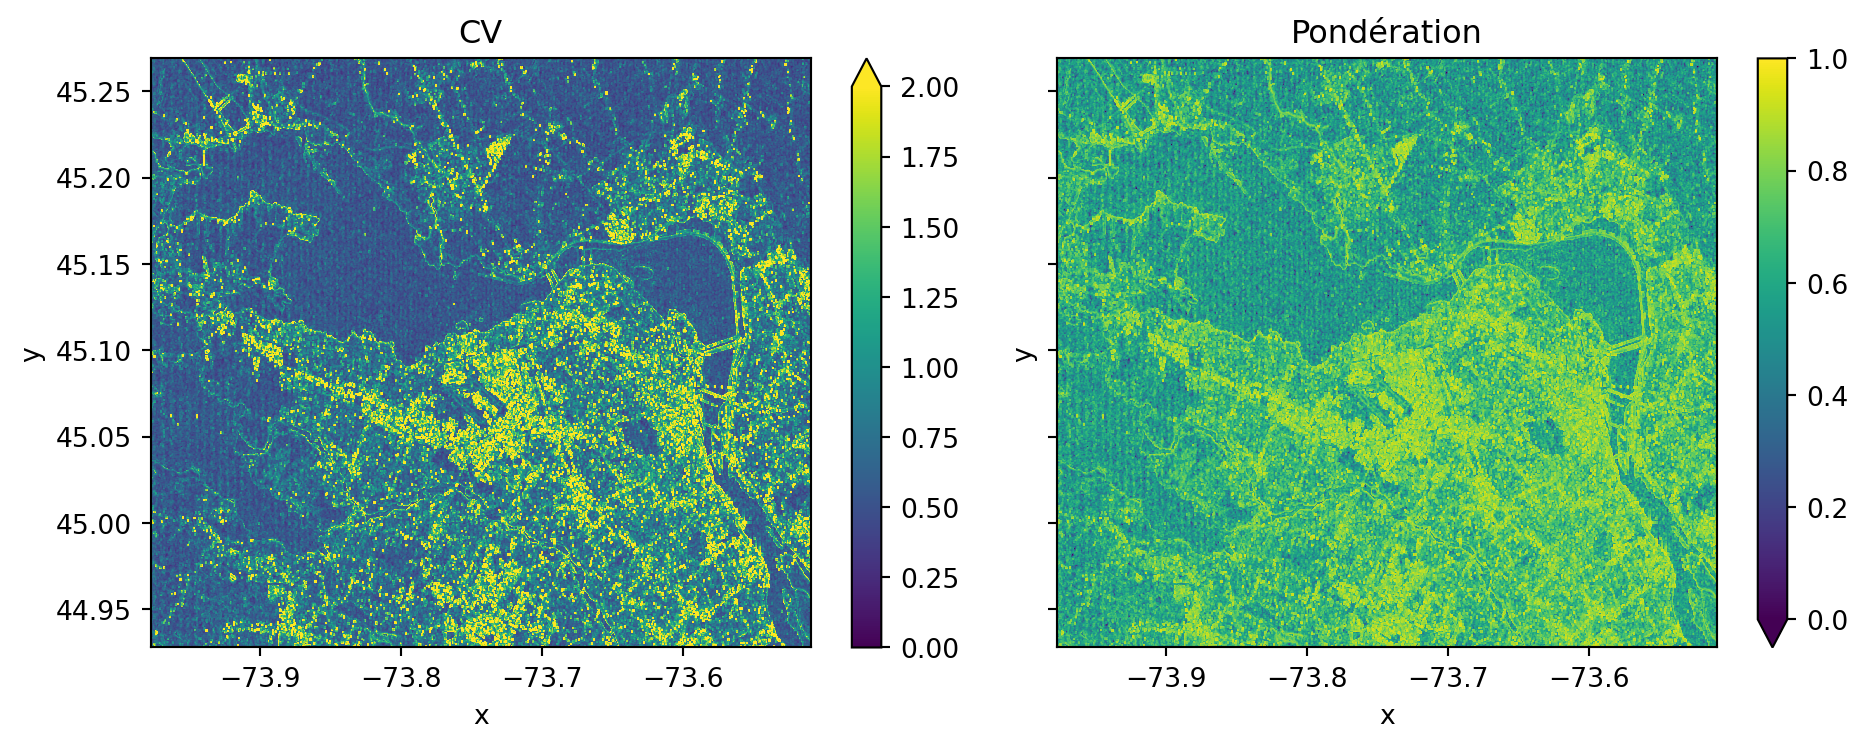
\includegraphics[width=9.72917in,height=3.89583in]{04-TransformationSpatiales_files/figure-html/cell-19-output-1.png}
\caption{}
\end{figure}

On zoomant sur l'image on peut clairement voir que les détails de
l'image sont mieux préservés:

\phantomsection\label{4c9224a6}
\begin{figure}
\centering
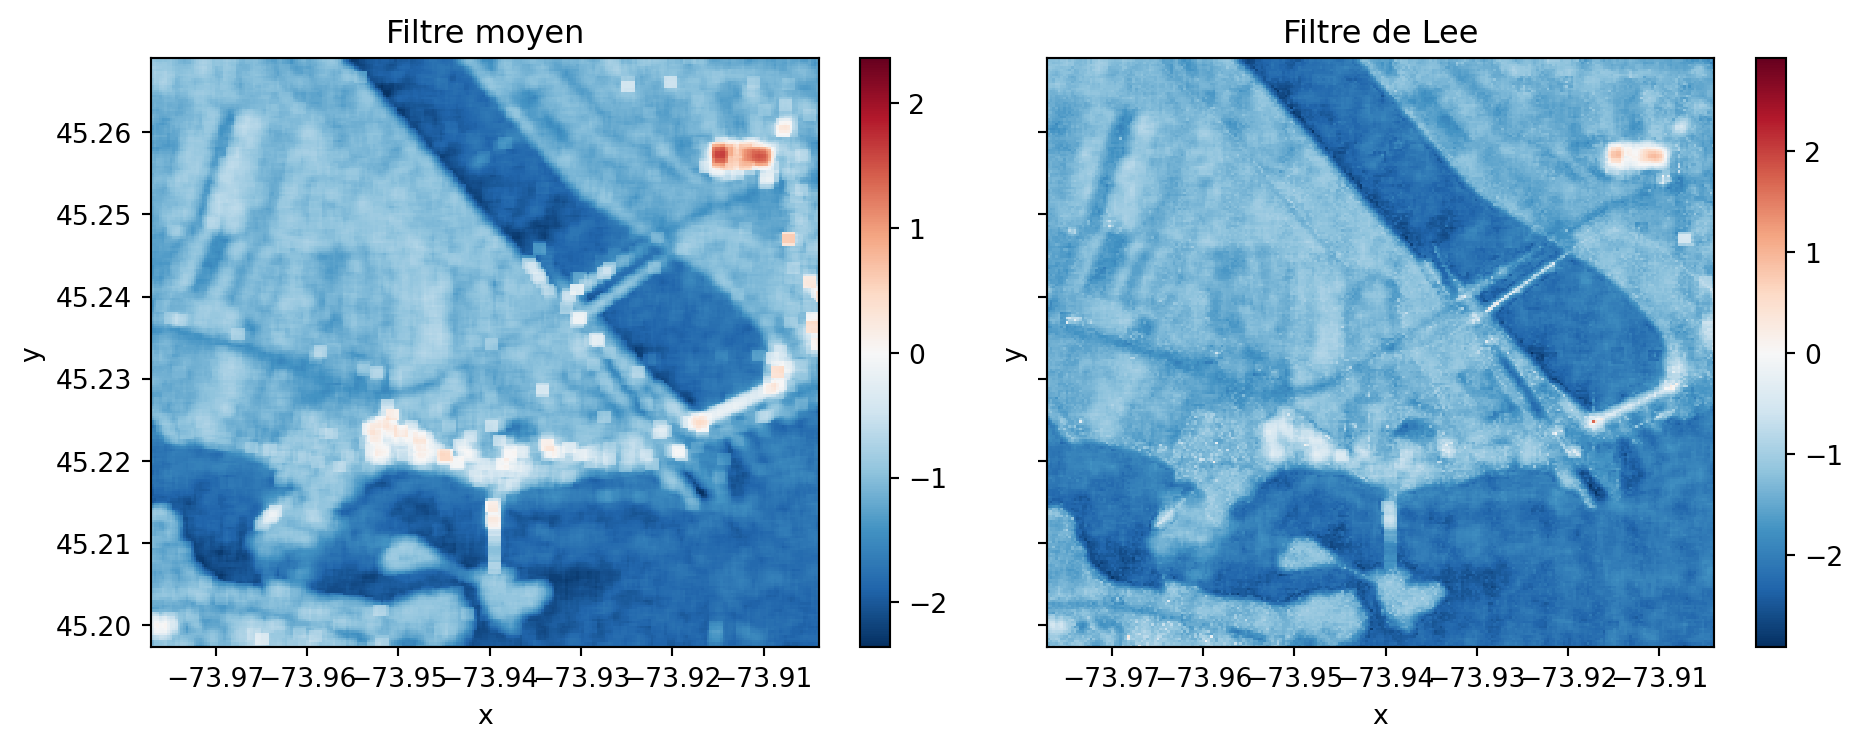
\includegraphics[width=9.69792in,height=3.89583in]{04-TransformationSpatiales_files/figure-html/cell-20-output-1.png}
\caption{}
\end{figure}

\subsection{\texorpdfstring{{5.4}
Segmentation}{5.4 Segmentation}}\label{segmentation}

La segmentation d'image consiste à séparer une image en régions
homogènes spatialement connexes (segments) où les valeurs sont uniformes
selon un certain critère (couleurs, texture, etc.). Une image présente
généralement beaucoup de pixels redondants, l'intérêt de ce type de
méthode est essentiellement de réduire la quantité de pxiels nécessaire.
En télédétection, on parle souvent d'approche objet. En vision par
ordinateur, on parle parfois de super-pixel. Il existe de nombreuses
méthodes de segmentation, la librairie \texttt{sickit-image} rend
disponible plusieurs implémentations sur des images RVB
(\href{https://scikit-image.org/docs/stable/auto_examples/segmentation/plot_segmentations.html\#sphx-glr-auto-examples-segmentation-plot-segmentations-py}{Comparison
of segmentation and superpixel algorithms --- skimage 0.25.0
documentation}).

\subsubsection{\texorpdfstring{{5.4.1}
Super-pixel}{5.4.1 Super-pixel}}\label{super-pixel}

Ce type de méthode cherche à former des régions homogènes et compactes
dans l'image {(\href{references.html\#ref-Achanta-2012}{Achanta et
Süsstrunk 2012})}. Une des méthodes les plus simples est la méthode SLIC
(\emph{Simple Linear Iterative Clustering}), elle combine un
regroupement de type K-moyenne avec une distance hybride qui prend en
compte les différences de couleur entre pixels mais aussi leur distance
par rapport centre du super-pixel:

\begin{enumerate}
\def\labelenumi{\arabic{enumi}.}
\item
  Décomposer l'image en N régions régulières de taille {\textbackslash(S
  \textbackslash times S\textbackslash)}
\item
  Initialiser les centres {\textbackslash(C\_k\textbackslash)} de chaque
  segment {\textbackslash(k\textbackslash)}
\item
  Rechercher les pixels qui ont la distance la plus petite dans une
  région {\textbackslash(2S \textbackslash times 2S\textbackslash)}:
\end{enumerate}

{\textbackslash{[} D\_\{SLIC\}= d\_\{couleur\} +
\textbackslash frac\{m\}\{S\}d\_\{xy\} \textbackslash{]}}

\begin{enumerate}
\def\labelenumi{\arabic{enumi}.}
\setcounter{enumi}{2}
\tightlist
\item
  Mettre à jour les centre {\textbackslash(C\_k\textbackslash)} de
  chaque segment {\textbackslash(k\textbackslash)}, retourner à l'étape
  3
\end{enumerate}

Les régions évoluent rapidement avec les itérations, plus le poids
{\textbackslash(m\textbackslash)} est élevé, plus la forme du
super-pixel est contrainte et ne suivra pas vraiment le contenu de
l'image:

\phantomsection\label{6032e407}
\phantomsection\label{cb29}
\begin{Shaded}
\begin{Highlighting}[]
\NormalTok{img }\OperatorTok{=}\NormalTok{ img\_rgb.to\_numpy().astype(}\StringTok{\textquotesingle{}uint8\textquotesingle{}}\NormalTok{).transpose(}\DecValTok{1}\NormalTok{,}\DecValTok{2}\NormalTok{,}\DecValTok{0}\NormalTok{) }

\NormalTok{segments\_slic1 }\OperatorTok{=}\NormalTok{ slic(img, n\_segments}\OperatorTok{=}\DecValTok{250}\NormalTok{, compactness}\OperatorTok{=}\DecValTok{10}\NormalTok{, sigma}\OperatorTok{=}\DecValTok{1}\NormalTok{, start\_label}\OperatorTok{=}\DecValTok{1}\NormalTok{, max\_num\_iter}\OperatorTok{=}\DecValTok{1}\NormalTok{)}
\NormalTok{segments\_slic2 }\OperatorTok{=}\NormalTok{ slic(img, n\_segments}\OperatorTok{=}\DecValTok{250}\NormalTok{, compactness}\OperatorTok{=}\DecValTok{10}\NormalTok{, sigma}\OperatorTok{=}\DecValTok{1}\NormalTok{, start\_label}\OperatorTok{=}\DecValTok{1}\NormalTok{, max\_num\_iter}\OperatorTok{=}\DecValTok{2}\NormalTok{)}
\NormalTok{segments\_slic100 }\OperatorTok{=}\NormalTok{ slic(img, n\_segments}\OperatorTok{=}\DecValTok{250}\NormalTok{, compactness}\OperatorTok{=}\DecValTok{100}\NormalTok{, sigma}\OperatorTok{=}\DecValTok{1}\NormalTok{, start\_label}\OperatorTok{=}\DecValTok{1}\NormalTok{, max\_num\_iter}\OperatorTok{=}\DecValTok{10}\NormalTok{)}
\NormalTok{segments\_slic100b }\OperatorTok{=}\NormalTok{ slic(img, n\_segments}\OperatorTok{=}\DecValTok{250}\NormalTok{, compactness}\OperatorTok{=}\DecValTok{10}\NormalTok{, sigma}\OperatorTok{=}\DecValTok{1}\NormalTok{, start\_label}\OperatorTok{=}\DecValTok{1}\NormalTok{, max\_num\_iter}\OperatorTok{=}\DecValTok{10}\NormalTok{)}

\BuiltInTok{print}\NormalTok{(}\SpecialStringTok{f\textquotesingle{}SLIC nombre de segments: }\SpecialCharTok{\{}\BuiltInTok{len}\NormalTok{(np.unique(segments\_slic1))}\SpecialCharTok{\}}\SpecialStringTok{\textquotesingle{}}\NormalTok{)}

\NormalTok{fig, ax }\OperatorTok{=}\NormalTok{ plt.subplots(}\DecValTok{2}\NormalTok{, }\DecValTok{2}\NormalTok{, figsize}\OperatorTok{=}\NormalTok{(}\DecValTok{10}\NormalTok{, }\DecValTok{6}\NormalTok{), sharex}\OperatorTok{=}\VariableTok{True}\NormalTok{, sharey}\OperatorTok{=}\VariableTok{True}\NormalTok{)}

\NormalTok{ax[}\DecValTok{0}\NormalTok{, }\DecValTok{0}\NormalTok{].imshow(mark\_boundaries(img, segments\_slic1))}
\NormalTok{ax[}\DecValTok{0}\NormalTok{, }\DecValTok{0}\NormalTok{].set\_title(}\StringTok{"Initialisation"}\NormalTok{)}
\NormalTok{ax[}\DecValTok{0}\NormalTok{, }\DecValTok{1}\NormalTok{].imshow(mark\_boundaries(img, segments\_slic2))}
\NormalTok{ax[}\DecValTok{0}\NormalTok{, }\DecValTok{1}\NormalTok{].set\_title(}\StringTok{\textquotesingle{}2 itérations\textquotesingle{}}\NormalTok{)}
\NormalTok{ax[}\DecValTok{1}\NormalTok{, }\DecValTok{0}\NormalTok{].imshow(mark\_boundaries(img, segments\_slic100))}
\NormalTok{ax[}\DecValTok{1}\NormalTok{, }\DecValTok{0}\NormalTok{].set\_title(}\StringTok{\textquotesingle{}10 itérations avec m=100\textquotesingle{}}\NormalTok{)}
\NormalTok{ax[}\DecValTok{1}\NormalTok{, }\DecValTok{1}\NormalTok{].imshow(mark\_boundaries(img, segments\_slic100b))}
\NormalTok{ax[}\DecValTok{1}\NormalTok{, }\DecValTok{1}\NormalTok{].set\_title(}\StringTok{\textquotesingle{}10 itérations avec m=10\textquotesingle{}}\NormalTok{)}

\ControlFlowTok{for}\NormalTok{ a }\KeywordTok{in}\NormalTok{ ax.ravel():}
\NormalTok{    a.set\_axis\_off()}

\NormalTok{plt.tight\_layout()}
\NormalTok{plt.show()}
\end{Highlighting}
\end{Shaded}

\begin{verbatim}
SLIC nombre de segments: 240
\end{verbatim}

\begin{figure}
\centering
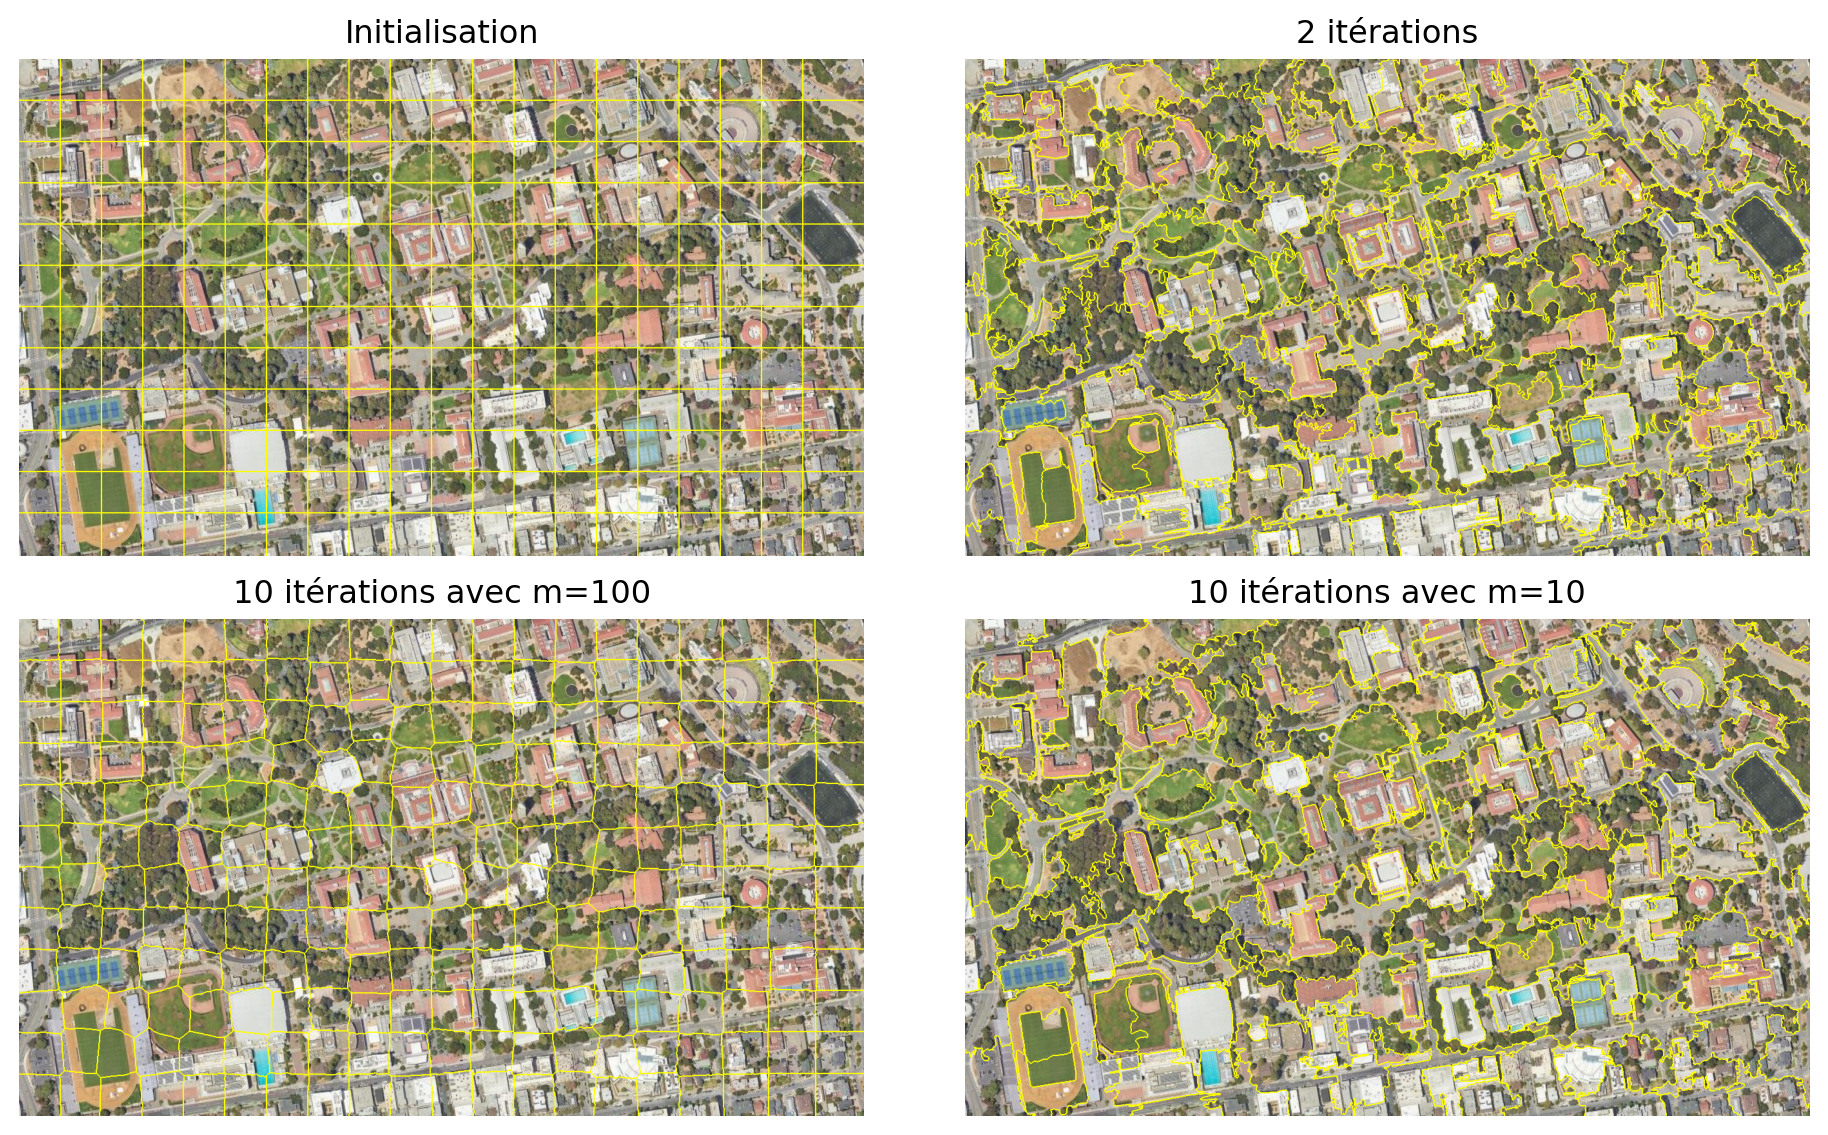
\includegraphics[width=9.52083in,height=5.91667in]{04-TransformationSpatiales_files/figure-html/cell-21-output-2.png}
\caption{}
\end{figure}

Le nombre de segments initial est probablement le paramètre le plus
important. Une manière de l'estimer est d'évaluer l'échelle moyenne des
segments homogènes dans l'image à analyser. On peut observer ci-dessous
l'impact de passer d'une échelle 40 x 40 à 20 x 20. En prenant la
moyenne de chaque segment, on peut voir tout de suite que 40 x 40
résulte en des segments trop grands mélangeant différentes classes.

\phantomsection\label{62d7cafa}
\phantomsection\label{cb31}
\begin{Shaded}
\begin{Highlighting}[]
\ImportTok{from}\NormalTok{ skimage }\ImportTok{import}\NormalTok{ color, segmentation}
\NormalTok{n\_regions }\OperatorTok{=} \BuiltInTok{int}\NormalTok{((img.shape[}\DecValTok{0}\NormalTok{] }\OperatorTok{*}\NormalTok{ img.shape[}\DecValTok{1}\NormalTok{])}\OperatorTok{/}\NormalTok{(}\DecValTok{40}\OperatorTok{*}\DecValTok{40}\NormalTok{))}
\BuiltInTok{print}\NormalTok{(}\StringTok{\textquotesingle{}Nb segments: \textquotesingle{}}\NormalTok{,n\_regions)}
\NormalTok{segments\_slic\_40 }\OperatorTok{=}\NormalTok{ slic(img, n\_segments}\OperatorTok{=}\NormalTok{n\_regions, compactness}\OperatorTok{=}\DecValTok{10}\NormalTok{, sigma}\OperatorTok{=}\DecValTok{1}\NormalTok{, start\_label}\OperatorTok{=}\DecValTok{1}\NormalTok{, max\_num\_iter}\OperatorTok{=}\DecValTok{10}\NormalTok{)}
\BuiltInTok{print}\NormalTok{(}\SpecialStringTok{f\textquotesingle{}SLIC nombre de segments: }\SpecialCharTok{\{}\BuiltInTok{len}\NormalTok{(np.unique(segments\_slic\_40))}\SpecialCharTok{\}}\SpecialStringTok{\textquotesingle{}}\NormalTok{)}
\NormalTok{out }\OperatorTok{=}\NormalTok{ color.label2rgb(segments\_slic\_40, img, kind}\OperatorTok{=}\StringTok{\textquotesingle{}avg\textquotesingle{}}\NormalTok{, bg\_label}\OperatorTok{=}\DecValTok{0}\NormalTok{)}
\NormalTok{out\_40 }\OperatorTok{=}\NormalTok{ segmentation.mark\_boundaries(out, segments\_slic\_40, (}\DecValTok{0}\NormalTok{, }\DecValTok{0}\NormalTok{, }\DecValTok{0}\NormalTok{))}

\NormalTok{n\_regions }\OperatorTok{=} \BuiltInTok{int}\NormalTok{((img.shape[}\DecValTok{0}\NormalTok{] }\OperatorTok{*}\NormalTok{ img.shape[}\DecValTok{1}\NormalTok{])}\OperatorTok{/}\NormalTok{(}\DecValTok{20}\OperatorTok{*}\DecValTok{20}\NormalTok{))}
\BuiltInTok{print}\NormalTok{(}\StringTok{\textquotesingle{}Nb segments: \textquotesingle{}}\NormalTok{,n\_regions)}
\NormalTok{segments\_slic\_20 }\OperatorTok{=}\NormalTok{ slic(img, n\_segments}\OperatorTok{=}\NormalTok{n\_regions, compactness}\OperatorTok{=}\DecValTok{10}\NormalTok{, sigma}\OperatorTok{=}\DecValTok{1}\NormalTok{, start\_label}\OperatorTok{=}\DecValTok{1}\NormalTok{, max\_num\_iter}\OperatorTok{=}\DecValTok{10}\NormalTok{)}
\BuiltInTok{print}\NormalTok{(}\SpecialStringTok{f\textquotesingle{}SLIC nombre de segments: }\SpecialCharTok{\{}\BuiltInTok{len}\NormalTok{(np.unique(segments\_slic\_20))}\SpecialCharTok{\}}\SpecialStringTok{\textquotesingle{}}\NormalTok{)}
\NormalTok{out }\OperatorTok{=}\NormalTok{ color.label2rgb(segments\_slic\_20, img, kind}\OperatorTok{=}\StringTok{\textquotesingle{}avg\textquotesingle{}}\NormalTok{, bg\_label}\OperatorTok{=}\DecValTok{0}\NormalTok{)}
\NormalTok{out\_20 }\OperatorTok{=}\NormalTok{ segmentation.mark\_boundaries(out, segments\_slic\_20, (}\DecValTok{0}\NormalTok{, }\DecValTok{0}\NormalTok{, }\DecValTok{0}\NormalTok{))}

\NormalTok{fig, ax }\OperatorTok{=}\NormalTok{ plt.subplots(}\DecValTok{2}\NormalTok{, }\DecValTok{1}\NormalTok{, figsize}\OperatorTok{=}\NormalTok{(}\DecValTok{6}\NormalTok{, }\DecValTok{8}\NormalTok{), sharex}\OperatorTok{=}\VariableTok{True}\NormalTok{, sharey}\OperatorTok{=}\VariableTok{True}\NormalTok{)}

\NormalTok{ax[}\DecValTok{0}\NormalTok{].imshow(out\_40)}
\NormalTok{ax[}\DecValTok{0}\NormalTok{].set\_title(}\StringTok{"Initialisation avec 631 segments"}\NormalTok{)}
\NormalTok{ax[}\DecValTok{1}\NormalTok{].imshow(out\_20)}
\NormalTok{ax[}\DecValTok{1}\NormalTok{].set\_title(}\StringTok{\textquotesingle{}Initialisation avec 2526 segments\textquotesingle{}}\NormalTok{)}
\ControlFlowTok{for}\NormalTok{ a }\KeywordTok{in}\NormalTok{ ax.ravel():}
\NormalTok{    a.set\_axis\_off()}
\NormalTok{plt.tight\_layout()}
\NormalTok{plt.show()}
\end{Highlighting}
\end{Shaded}

\begin{verbatim}
Nb segments:  631
SLIC nombre de segments: 459
Nb segments:  2526
SLIC nombre de segments: 2201
\end{verbatim}

\begin{figure}
\centering
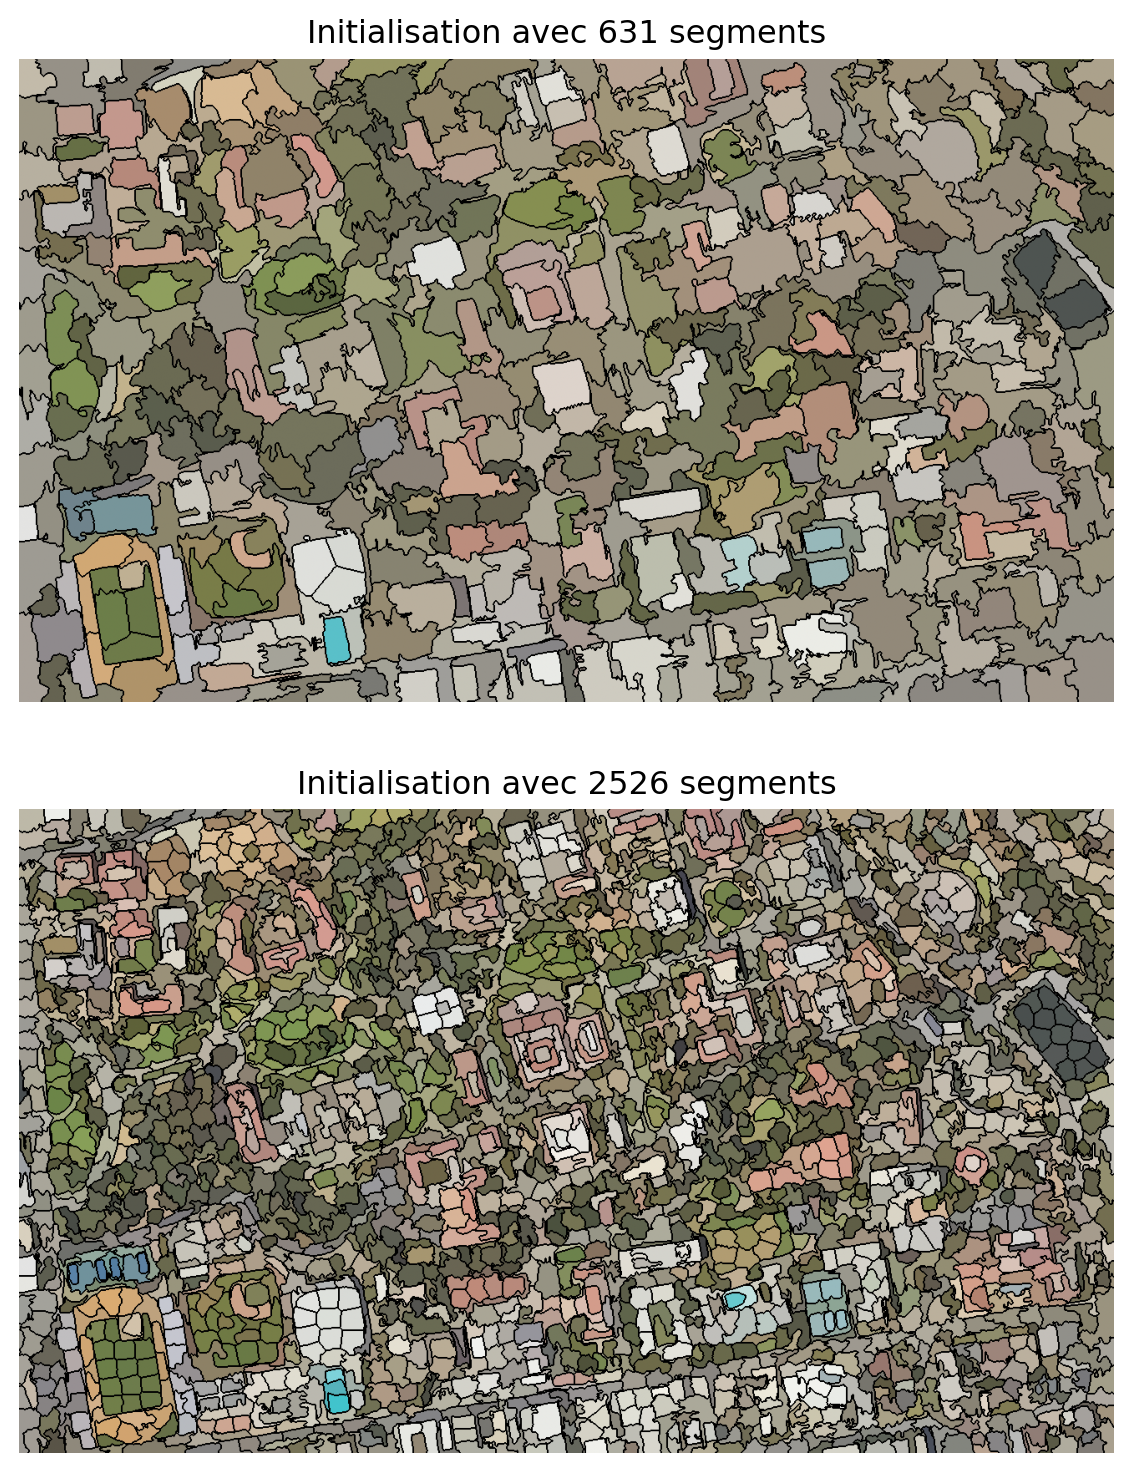
\includegraphics[width=5.89583in,height=7.66667in]{04-TransformationSpatiales_files/figure-html/cell-22-output-2.png}
\caption{}
\end{figure}

\subsubsection{\texorpdfstring{{5.4.2} Fusion des segments par graphe de
proximité}{5.4.2 Fusion des segments par graphe de proximité}}\label{fusion-des-segments-par-graphe-de-proximituxe9}

Une segmentation peut produire beaucoup trop de segments. On parle alors
de sur-segmentation. Ceci est recherché dans certains cas pour permettre
de bien capturer les détails fins de l'image. Cependant, afin de réduire
le nombre de segments, un post-traitement possible est de fusionner les
segments similaires selon certaines règles ou distances. Un graphe
d'adjacence de régions (voir \hyperref[fig-rag]{figure~{5.1}}) est formé
à partir des segments connectés où chaque noeud représente un segment et
un lien une proximité ({Jaworek-Korjakowska
(\href{references.html\#ref-Jaworek-2018}{2018})}). À partir de ce
graphe, on peut fusionner les noeuds similaires à partir de leur
distance radiométrique.

\phantomsection\label{fig-rag}
\begin{figure}
\centering
\pandocbounded{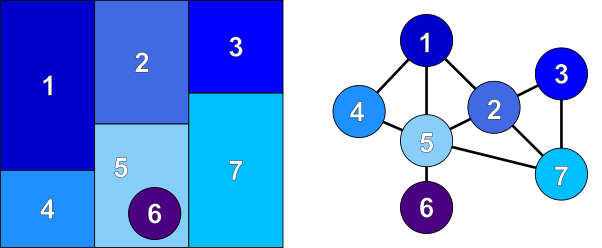
\includegraphics[keepaspectratio]{images/Region-adjacency-graph.png}}
\caption{Figure~5.1: Graphe d'adjacence de régions, d'après
({Jaworek-Korjakowska
(\href{references.html\#ref-Jaworek-2018}{2018})}). Chaque noeud est un
segment, un lien est formé uniquement si les segments se touchent (par
exemple le segment 6 ne touche que la région 5). La fonction
\texttt{graph.rag\_mean\_color} produit un graphe à partir d'une
segmentation et de l'image originale. Chaque noeud tient la couleur de
chaque segment dans un attribut appelé
\texttt{\textquotesingle{}mean\ color\textquotesingle{}.}}
\end{figure}

\phantomsection\label{546ab572}
\phantomsection\label{cb33}
\begin{Shaded}
\begin{Highlighting}[]
\KeywordTok{def}\NormalTok{ \_weight\_mean\_color(graph, src, dst, n):}
    \CommentTok{"""Fonction pour gérer la fusion des nœuds en recalculant la couleur moyenne.}
\CommentTok{    La méthode suppose que la couleur moyenne de \textasciigrave{}dst\textasciigrave{} est déjà calculée.}
\CommentTok{    """}
\NormalTok{    diff }\OperatorTok{=}\NormalTok{ graph.nodes[dst][}\StringTok{\textquotesingle{}mean color\textquotesingle{}}\NormalTok{] }\OperatorTok{{-}}\NormalTok{ graph.nodes[n][}\StringTok{\textquotesingle{}mean color\textquotesingle{}}\NormalTok{]}
\NormalTok{    diff }\OperatorTok{=}\NormalTok{ np.linalg.norm(diff)}
    \CommentTok{\#print(diff)}
    \ControlFlowTok{return}\NormalTok{ \{}\StringTok{\textquotesingle{}weight\textquotesingle{}}\NormalTok{: diff\}}


\KeywordTok{def}\NormalTok{ merge\_mean\_color(graph, src, dst):}
    \CommentTok{"""Fonction appelée avant la fusion de deux nœuds d\textquotesingle{}un graphe de distance de couleur moyenne.}
\CommentTok{      Cette méthode calcule la couleur moyenne de \textasciigrave{}dst\textasciigrave{}.}
\CommentTok{    """}
\NormalTok{    graph.nodes[dst][}\StringTok{\textquotesingle{}total color\textquotesingle{}}\NormalTok{] }\OperatorTok{+=}\NormalTok{ graph.nodes[src][}\StringTok{\textquotesingle{}total color\textquotesingle{}}\NormalTok{]}
\NormalTok{    graph.nodes[dst][}\StringTok{\textquotesingle{}pixel count\textquotesingle{}}\NormalTok{] }\OperatorTok{+=}\NormalTok{ graph.nodes[src][}\StringTok{\textquotesingle{}pixel count\textquotesingle{}}\NormalTok{]}
\NormalTok{    graph.nodes[dst][}\StringTok{\textquotesingle{}mean color\textquotesingle{}}\NormalTok{] }\OperatorTok{=}\NormalTok{ (}
\NormalTok{        graph.nodes[dst][}\StringTok{\textquotesingle{}total color\textquotesingle{}}\NormalTok{] }\OperatorTok{/}\NormalTok{ graph.nodes[dst][}\StringTok{\textquotesingle{}pixel count\textquotesingle{}}\NormalTok{]}
\NormalTok{    )}
\NormalTok{g }\OperatorTok{=}\NormalTok{ graph.rag\_mean\_color(img, segments\_slic\_20)}
\BuiltInTok{print}\NormalTok{(}\StringTok{\textquotesingle{}Nombre de segments:\textquotesingle{}}\NormalTok{,}\BuiltInTok{len}\NormalTok{(g))}
\NormalTok{labels2 }\OperatorTok{=}\NormalTok{ graph.merge\_hierarchical(}
\NormalTok{    segments\_slic\_20,}
\NormalTok{    g,}
\NormalTok{    thresh}\OperatorTok{=}\DecValTok{20}\NormalTok{,}
\NormalTok{    rag\_copy}\OperatorTok{=}\VariableTok{False}\NormalTok{,}
\NormalTok{    in\_place\_merge}\OperatorTok{=}\VariableTok{True}\NormalTok{,}
\NormalTok{    merge\_func}\OperatorTok{=}\NormalTok{merge\_mean\_color,}
\NormalTok{    weight\_func}\OperatorTok{=}\NormalTok{\_weight\_mean\_color,}
\NormalTok{)}
\BuiltInTok{print}\NormalTok{(}\StringTok{\textquotesingle{}Nombre de segments:\textquotesingle{}}\NormalTok{,}\BuiltInTok{len}\NormalTok{(g))}

\NormalTok{out1 }\OperatorTok{=}\NormalTok{ color.label2rgb(segments\_slic\_20, img, kind}\OperatorTok{=}\StringTok{\textquotesingle{}avg\textquotesingle{}}\NormalTok{, bg\_label}\OperatorTok{=}\DecValTok{0}\NormalTok{)}
\NormalTok{out1 }\OperatorTok{=}\NormalTok{ segmentation.mark\_boundaries(out1, segments\_slic\_20, (}\DecValTok{0}\NormalTok{, }\DecValTok{0}\NormalTok{, }\DecValTok{0}\NormalTok{))}
\NormalTok{out2 }\OperatorTok{=}\NormalTok{ color.label2rgb(labels2, img, kind}\OperatorTok{=}\StringTok{\textquotesingle{}avg\textquotesingle{}}\NormalTok{, bg\_label}\OperatorTok{=}\DecValTok{0}\NormalTok{)}
\NormalTok{out2 }\OperatorTok{=}\NormalTok{ segmentation.mark\_boundaries(out2, labels2, (}\DecValTok{0}\NormalTok{, }\DecValTok{0}\NormalTok{, }\DecValTok{0}\NormalTok{))}

\NormalTok{fig, ax }\OperatorTok{=}\NormalTok{ plt.subplots(nrows}\OperatorTok{=}\DecValTok{2}\NormalTok{, sharex}\OperatorTok{=}\VariableTok{True}\NormalTok{, sharey}\OperatorTok{=}\VariableTok{True}\NormalTok{, figsize}\OperatorTok{=}\NormalTok{(}\DecValTok{6}\NormalTok{, }\DecValTok{8}\NormalTok{))}

\NormalTok{ax[}\DecValTok{0}\NormalTok{].imshow(out1)}
\NormalTok{ax[}\DecValTok{0}\NormalTok{].set\_title(}\StringTok{"Avant fusion"}\NormalTok{)}
\NormalTok{ax[}\DecValTok{1}\NormalTok{].imshow(out2)}
\NormalTok{ax[}\DecValTok{1}\NormalTok{].set\_title(}\StringTok{"Après fusion"}\NormalTok{)}
\ControlFlowTok{for}\NormalTok{ a }\KeywordTok{in}\NormalTok{ ax:}
\NormalTok{    a.axis(}\StringTok{\textquotesingle{}off\textquotesingle{}}\NormalTok{)}

\NormalTok{plt.tight\_layout()}
\end{Highlighting}
\end{Shaded}

\begin{verbatim}
Nombre de segments: 2201
Nombre de segments: 1187
\end{verbatim}

\begin{figure}
\centering
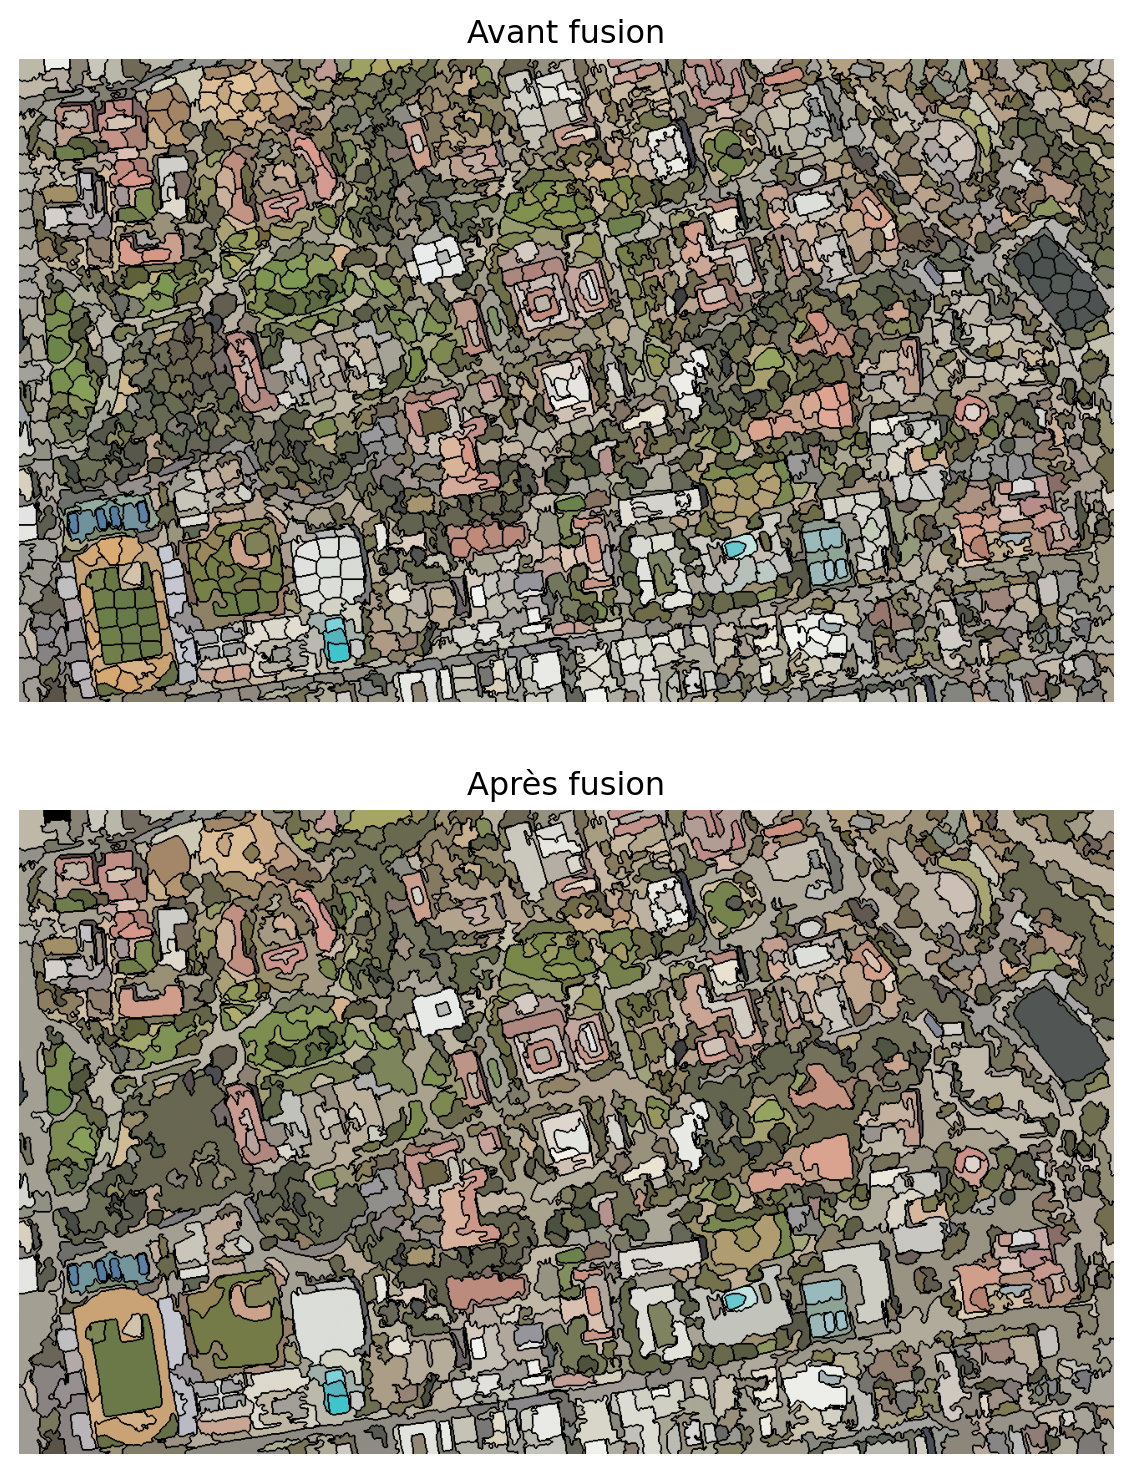
\includegraphics[width=5.89583in,height=7.67708in]{04-TransformationSpatiales_files/figure-html/cell-23-output-2.png}
\caption{}
\end{figure}

\subsubsection{\texorpdfstring{{5.4.3} Approche
objet}{5.4.3 Approche objet}}\label{approche-objet}

L'approche objet consiste à traiter chaque segment comme un objet avec
un ensemble de propriétés. La librairie \texttt{skimage} offre la
possibilité d'enrichir chaque segment avec des
\href{https://scikit-image.org/docs/stable/api/skimage.measure.html\#skimage.measure.regionprops}{propriétés}
et de former un tableau:

\phantomsection\label{f21073f1}
\phantomsection\label{cb35}
\begin{Shaded}
\begin{Highlighting}[]
\NormalTok{properties }\OperatorTok{=}\NormalTok{ [}\StringTok{\textquotesingle{}label\textquotesingle{}}\NormalTok{, }\StringTok{\textquotesingle{}area\textquotesingle{}}\NormalTok{, }\StringTok{\textquotesingle{}centroid\textquotesingle{}}\NormalTok{, }\StringTok{\textquotesingle{}num\_pixels\textquotesingle{}}\NormalTok{, }\StringTok{\textquotesingle{}intensity\_mean\textquotesingle{}}\NormalTok{, }\StringTok{\textquotesingle{}intensity\_std\textquotesingle{}}\NormalTok{]}

\NormalTok{table}\OperatorTok{=}\NormalTok{   measure.regionprops\_table(labels2, intensity\_image}\OperatorTok{=}\NormalTok{ img\_rgb.to\_numpy().transpose(}\DecValTok{1}\NormalTok{,}\DecValTok{2}\NormalTok{,}\DecValTok{0}\NormalTok{), properties}\OperatorTok{=}\NormalTok{properties)}

\NormalTok{table }\OperatorTok{=}\NormalTok{ pd.DataFrame(table)}
\NormalTok{table.head(}\DecValTok{10}\NormalTok{)}
\end{Highlighting}
\end{Shaded}

\begin{longtable}[]{@{}llllllllllll@{}}
\toprule\noalign{}
& label & area & centroid-0 & centroid-1 & num\_pixels &
intensity\_mean-0 & intensity\_mean-1 & intensity\_mean-2 &
intensity\_std-0 & intensity\_std-1 & intensity\_std-2 \\
\midrule\noalign{}
\endhead
\bottomrule\noalign{}
\endlastfoot
0 & 1 & 641.0 & 15.466459 & 69.489860 & 641 & 136.730103 & 132.851791 &
117.126366 & 32.289547 & 31.451048 & 37.421638 \\
1 & 2 & 480.0 & 10.997917 & 92.614583 & 480 & 201.208328 & 198.262497 &
188.483337 & 14.184592 & 14.151334 & 15.475913 \\
2 & 3 & 712.0 & 16.683989 & 114.776685 & 712 & 185.349716 & 183.113770 &
170.994385 & 25.453747 & 26.184948 & 28.128426 \\
3 & 4 & 1803.0 & 31.974487 & 139.379368 & 1803 & 117.897392 & 108.367722
& 97.769829 & 31.086676 & 26.577900 & 28.297256 \\
4 & 5 & 448.0 & 5.004464 & 166.542411 & 448 & 183.511154 & 181.276779 &
167.720978 & 29.824030 & 30.625013 & 31.297607 \\
5 & 6 & 459.0 & 9.934641 & 191.668845 & 459 & 133.557739 & 133.821350 &
129.697174 & 22.902142 & 23.013086 & 22.428919 \\
6 & 7 & 355.0 & 5.160563 & 222.895775 & 355 & 148.574646 & 148.802811 &
142.580276 & 21.334805 & 21.457472 & 20.931572 \\
7 & 8 & 334.0 & 4.904192 & 255.904192 & 334 & 125.973053 & 121.197601 &
108.973053 & 23.151978 & 24.556480 & 25.351229 \\
8 & 9 & 1481.0 & 32.279541 & 292.865631 & 1481 & 204.102631 & 172.359894
& 137.501007 & 13.884891 & 14.092896 & 15.865581 \\
9 & 10 & 445.0 & 8.013483 & 308.053933 & 445 & 145.373032 & 138.182022 &
121.402245 & 18.543356 & 18.644655 & 22.237881 \\
\end{longtable}

Ce tableau pourra être exploiter pour une tâche de classification par la
suite (on parle alors de classification objet).

\phantomsection\label{refs}
\begin{CSLReferences}{1}{0}
\bibitem[\citeproctext]{ref-Achanta-2012}
Achanta, Kevin Smith adhakrishna, Appu Shaji et Sabine Süsstrunk. 2012.
{«~SLIC Superpixels Compared to State-of-the-art Superpixel Methods.~»}
\emph{{TPAMI}}: 636‑643. \url{https://doi.org/10.1109/TPAMI.2012.120}.

\bibitem[\citeproctext]{ref-Cooley-1965}
Cooley, James W. et John W. Tukey. 1965. {«~An algorithm for the machine
calculation of complex Fourier series.~»} \emph{{Math. Comput.}}:
297‑301.
\url{https://web.stanford.edu/class/cme324/classics/cooley-tukey.pdf}.

\bibitem[\citeproctext]{ref-Scharr1999}
Jahne, Scharr, B et Korkel S. 1999. \emph{Principles of filter design}.
Handbook of Computer Vision; Applications; Academic Press.

\bibitem[\citeproctext]{ref-Jaworek-2018}
Jaworek-Korjakowska, P., J.; Kłeczek. 2018. {«~Region Adjacency Graph
Approach for Acral Melanocytic Lesion Segmentation.~»} \emph{{Applied
Sciences}} 8: 1430.
\href{https://10.3390/app8091430}{10.3390/app8091430}.

\bibitem[\citeproctext]{ref-Lee-1986}
Lee, J. S. 1986. {«~Speckle suppression and analysis for synthetic
aperture radar images.~»} \emph{{Opt. Eng.}} 25 (5): 636‑643.
\url{https://doi.org/10.1117/12.7973877}.

\end{CSLReferences}

\end{document}
